\documentclass[12pt, oneside]{report}
\usepackage{amsmath}
\usepackage{amssymb}
\usepackage{amsthm}
\usepackage{graphicx}
\usepackage{color}
\usepackage{hyperref}
\usepackage{enumerate}

\usepackage{url}
\author{}

\setcounter{tocdepth}{1}

\usepackage{hyphenat}
\usepackage[T1, T2A]{fontenc}
\usepackage[utf8]{inputenc}
\usepackage[main=bulgarian, english, japanese]{babel}
\usepackage{CJKutf8}

\usepackage{array}
\usepackage{tabularx}
\usepackage{caption}
\usepackage{longtable}

\let\cleardoublepage\clearpage

% \usepackage{fontspec}
% \setmainfont{CMU Serif}
% \setsansfont{CMU Sans Serif}
% \setmonofont{CMU Typewriter Text}

% \usepackage{xeCJK}
% \setCJKmainfont{ipam.ttf}
% \setCJKsansfont{ipag.ttf}

\selectbglanguage
\setlocalecaption{bulgarian}{contents}{Съдържание}
\setlocalecaption{bulgarian}{chaptername}{Глава}
\usepackage[toc, page, titletoc,title]{appendix}
\usepackage{pdfpages}

\title{ТРУДОВ РЕЧНИК\\
\large{Японски и китайски имена, английски, военни и спортни термини}}

\begin{document}

\maketitle

\selectbglanguage

\section*{Благодарности}
    
Благодарности за изготвянето на речника: Ragnos и postmortem от Eastern Spirit, KoP3Le7o, DARK RANGER, Alexeev, nightwarrior, Chep\_92, Hristo Lishev, BestRipper, Stone, simo76, Анубис, Phoebes, Ice-Man, D300, elisiaelf, SonGoku, ludoto\_mimi, shtipliiska, danissimo, \-\=\ F\ o\ z\ z\ y\ \=\-, Zaza14, Николай, riburan, ex-cuckoo, kelly, spotbeam, pinko™, kaloo, rburan, fakelini, motleycrue, burndead, milenski, freakazoid, star6inkata, sed, tnt1918, mass\_effect, cheeseus, Скуби Ду, o6ina, Guilty, dkp

\quad

Информацията е събрана в периода 2013-2015 г.

\quad

Графично оформление от Rinto-kun.

\tableofcontents

\listoftables

\chapter{Японски имена}
\label{chap:imena}
\section{Основни правила при транскрипцията на японски имена}
\subsection{Дългите гласни}
В практическата транскрипция е прието \textbf{дължината на гласните} да не се предава.
Когато обаче йероглифният запис на \textbf{съответното име} или \textbf{термин} е даден в скобки, той може да бъде \textbf{транскрибиран на кирилица}, като се отрази и дължината на гласните.
Затова например глинените фигурки от \textit{периода Джьомон} в текста се срещат като \textit{догу}, но йероглифният запис е транскрибиран като \textit{догуу}.

Аналогичен е случаят и с термина \textit{шинто}, който всъщност звучи като \textit{шинтоо}.
При необходимост предаването на дългите гласни може да стане по няколко начина: чрез повторно изписване на съответната гласна; чрез чертица над буквата; чрез двоеточие след нея. Така дългата гласна \textbf{/a/} може да се срещне като \textbf{/aa, \-а, a:/}.
В англоезичната литература е разпространено и предаването на дължината с помощта на буквата h. Така например названието на \textit{японския театър Но}, което в действителност звучи \textbf{/ноо/},
на английски се транскрибира като \textbf{Noh}.

\subsection{Редукция на гласните}
Типична за японския език е редукцията на тесните гласни \textbf{/u, i/} в неударени срички и в края на думите, както е например в \textbf{копулата /десу/} и в \textbf{суфикса /масу/}.
Тъй като в тези случаи \textbf{редукцията} е почти пълна, при предаване на японски имена с наставка \textbf{суке}, е по-добре тя да се изписва като \textbf{ске}, т.е \textit{Дайске}, а не \textit{Дайсуке}.

\subsection{Двойните съгласни}
Двойните съгласни се предават при свързването на \textbf{две морфеми} и при т.нар. \textbf{експресивна геминация}. Името на страната може да бъде произнесено или като \textit{Нихон}, или като \textit{Ниппон}, но не и като \textit{Нипон}. Важно е да се знае, че \textit{Нихон} и \textit{Ниппон} не са напълно взаимозаменяеми.
Например в спортни призиви при международни мачове се използва \textit{„Ниппон – Ганбаре Ниппон“}!

В японския се среща\textbf{ удвояване на съгласните}, което в английската транскрипция се отбелязва
просто с \textbf{удвоение на буквите}, като например \textbf{"kk"}, \textbf{"tt"}. Това се прави и в българската транскрипция. Т.е. в такива случаи се транслитерира буквално - \textbf{tt = тт, kk = кк}, и т.н.

\subsection{Морообразуващата съгласна /н/}
В японски език се срещат \textbf{два вида съгласни /н/}. Едната не се различава от българската и в позиция пред букви, предаващи йотувани гласни, се смекчава. Другата, която се записва с буквата \begin{CJK*}{UTF8}{song}ん\end{CJK*}, е т.нар. \textbf{морообразуваща съгласна /н/}, която винаги се \textbf{произнася като} \textbf{твърда}. В английската транскрипция този звук се предава чрез \textbf{апостроф (n’),} както в заглавието на антологията \textbf{Man’y\-osh\-u}, ако е отразена дължината на гласните, и като \textbf{Man’yoshu}, ако не е отразена.
В руската транскрипция се използва буквата \textbf{\"e}, която се нарича \textbf{твердый знак} и при необходимост изпълнява ролята на \textbf{апостроф}, както например в \textbf{Манъ\"eсю}.
В българската азбука \textbf{ъ} има самостоятелна звукова стойност и не може да се използва като апостроф. Тъй като употребата на апостроф, макар и с по-други функции, се допуска от българския правопис, тук ще го използвам в съчетание с буквата \textbf{н} за предаване на морообразуващата съгласна, както например \textbf{Ман’йошю}.

\subsection{Меките ж, ч, ш}
Българският правоговор изисква съгласните \textbf{ж, ч, ш} да се произнасят като \textbf{твърди}, но в японския език те са \textbf{меки съгласни}. Сричката 
\begin{CJK*}{UTF8}{song}しゅ\end{CJK*} например се предава или като \textbf{шу} под влияние на английската транскрипция, или като \textbf{сю} под влияние на руската. По-близо до японското произношение обаче е \textbf{шю}. Ето защо името на най-големия японски остров например е \textbf{Хоншю}, а не \textbf{Хоншу} или \textbf{Хонсю}.

\subsection{Дзен или зен}
Под влияние на \textbf{английската транскрипция} често се пише \textbf{з} вместо \textbf{дз}, като дори се твърди, че това е правилното произношение. Ако обаче привържениците на това твърдение помолят някой японец да произнесе например думата \textbf{защо}, със сигурност ще чуят \textbf{дзащо}.

\subsection{Сричката /цу/}
Африкатата \textbf{/ц/,} която се среща в японската сричка \textbf{/цу/,} при транскрипция с латиница се предава с буквосъчетанието \textbf{/ts/.} Тъй като този звук не се различава от българския \textbf{/ц/,} \textbf{при} \textbf{транскрибирането} му не би трябвало да има колебания.
Но авторите, които \textbf{механично следват английската транскрипция}, често пишат или\textbf{ тс, }или\textbf{ }дори\textbf{ тц}. Така \textbf{Цукуба} се среща и като \textbf{Тсукуба}, и като \textbf{Тцукуба}. \\\\

\textbf{Източник:} „\textbf{\textit{Японската цивилизация}}“ от Братислав Иванов.
 
\begin{table}[htbp]
    \centering
    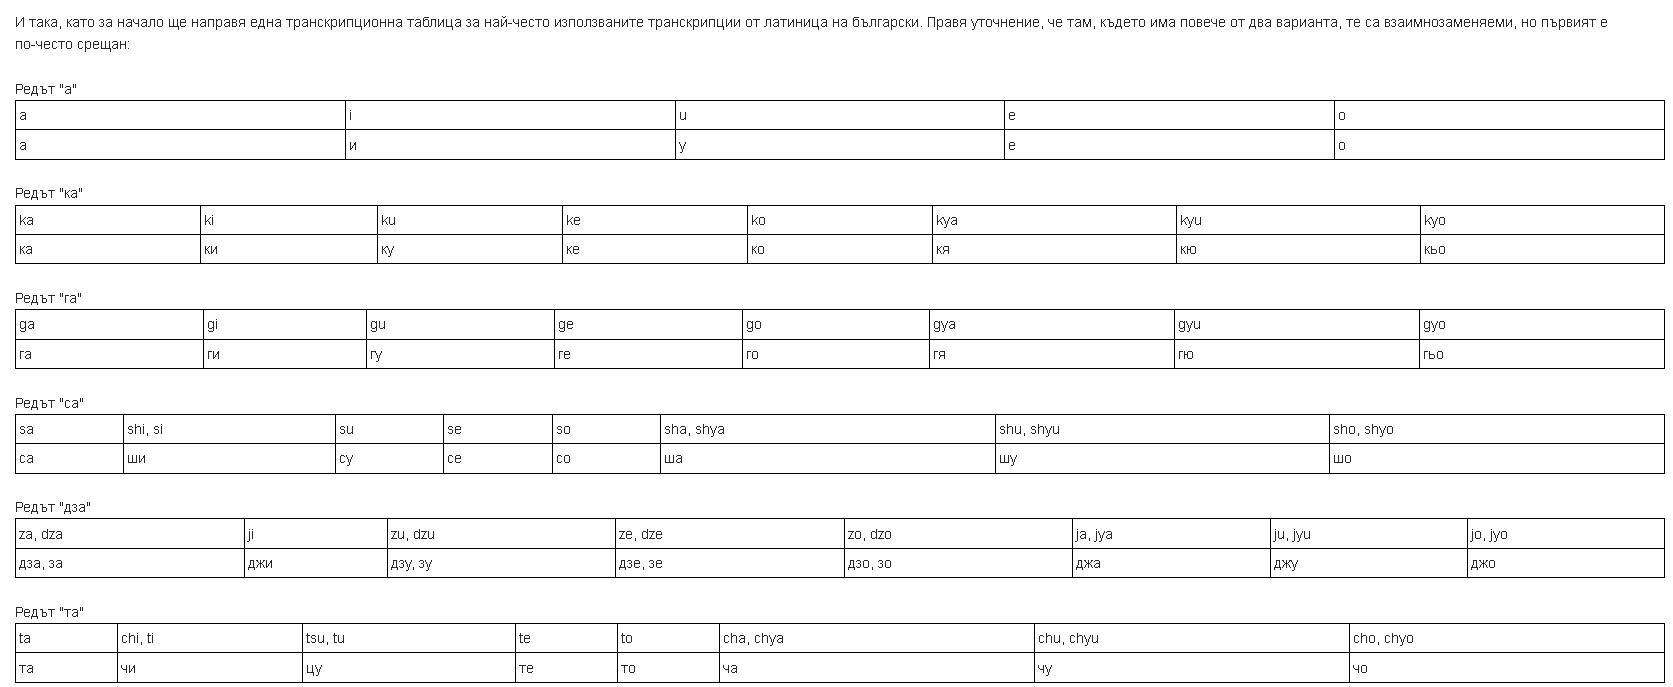
\includegraphics[width=\textwidth]{chapters/transcription-1.JPG}
    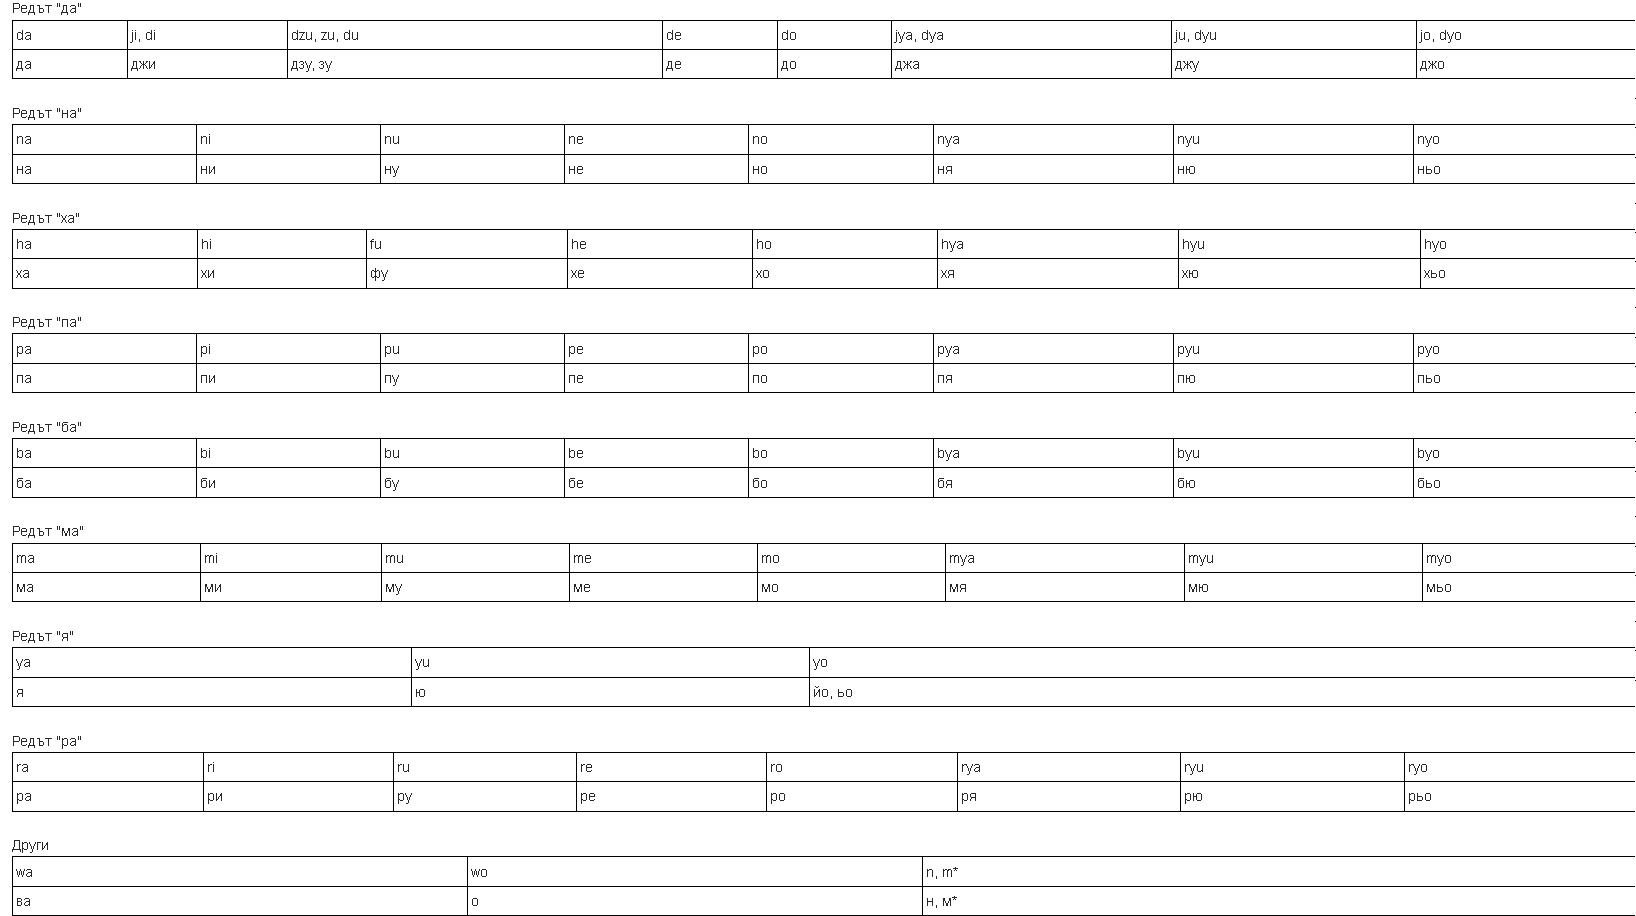
\includegraphics[width=\textwidth]{chapters/transcription-2.JPG}
    \caption{Транскрипционна таблица}
\end{table}

\clearpage

\section{Японски език за българи}
Следващата част е извадена от учебното пособие „Японски език за българи“ от Атанас Атанасов и Томоки Ватанабе.

\includepdf[pages={2-6},lastpage=24]{textbook.pdf} 
  

\chapter{Японски обръщения}
В тази част смятам да поясня малко повече за обръщенията, които се използват
в японския език и \textbf{как} и \textbf{дали} да ги \textbf{превеждаме}. Като начало трябва да се каже,
че ако се превеждат тези обръщения, никак не е уместно да се ползват множеството обръщения, навлезли от английски, френски и т.н. от сорта на "\textbf{сър}", "\textbf{мистър}", "\textbf{мадам}" и т.н.,
\textbf{освен ако контекстът изрично не го изисква}. Също трябва да спомена, че някои от обръщенията
са \textbf{непреводими} и ако държите да превеждате обръщенията, просто ще се наложи да ги пропускате.

\section{Често срещани}
\begin{longtable}{|p{0.2\textwidth}|p{0.8\textwidth}|}
\hline
\textbf{Наставка} & \textbf{Превод} \\ \hline
\endfirsthead
\hline
\endhead
\hline
\endfoot

\textbf{-san}& г-н, г-жа, г-жица \\
\textbf{-chan/-kun}& практически \textbf{непреводимо}, оставяте само името \\
\textbf{-sama/-dono}& господарю, господарке (понякога се използват с ироничен привкус и тогава може да използвате различни вариации като \textbf{,,всемогъщи''}, \textbf{,,вездесъщи''} и т.н., но \textbf{само в шеговит контекст}) \\
-\textbf{sempai}& може да се каже, че е непреводимо, евентуално може като \textbf{,,старши''}, но \textbf{само ако става въпрос за отношения на работното място}, например \\
\textbf{-kouhai}& по-неопитен и по-низш в йерархията, няма адекватен превод \\
\textbf{-sensei}& евентуално може да се преведе като \textbf{,,учителю''}, но съветвам и тук по-скоро да се оставя само името, тъй като \textbf{това обръщение се използва и за лекари, професори и т.н.} \\
\textbf{-senshuu}& за спортисти, евентуално като \textbf{,,състезател''}, или в зависимост от спорта, за който става въпрос. \\

\hline\caption{Основни обръщения в японския език}

\end{longtable}

\section{Фамилни имена}

\begin{table}[htbp]
    \centering
        \begin{tabular}{|p{0.15\textwidth}|p{0.85\textwidth}|}
            \hline
            \textbf{Наставка} & \textbf{Превод} \\ \hline
            \textbf{okaa-san / kaa-san}&майка, мамо\\ 
        \textbf{otou-san / tou-san}&татко, тате\\ 
        \textbf{onee-san / nee-san}&кака, како (както и в българския, може да се обръщат с "како" и към по-голямо момиче, което не е в семейството, но им е близко)\\ 
        \textbf{onii-san / nii-san}&батко, бате (казаното за \textbf{onee-san} важи и тук)\\ 
        \textbf{otouto}&по-малък брат, братче (тъй като в българския нямаме определена дума за това ви предлагам да не го превждате навсякъде където се споменава, а да го замествате с име или местоимение)\\ 
        \textbf{imouto}&по-малка сестра, сестричка (казаното за "otouto" важи и тук)\\ 
        \textbf{ojii-san / jii-san}&дядо (спокойно се използва и за хора извън семейството, както и в български)\\ 
        \textbf{obaa-san / baa-san}&баба, бабо (и това също се използва за хора извън семейството)\\ 
        \textbf{oji-san}&чичо\\ 
        \textbf{oba-san}&леля, лельо (и ,,чичо'', и ,,лельо'' пак са обръщения, които могат да се използват към хора, които не са роднини)\\ 
        
        \hline
        \end{tabular}
    \caption{Фамилни имена}
    \label{tab:familynames}
\end{table}

Както е видно, с изключение на \textbf{,,майка''} и \textbf{,,татко''}, всички други могат да бъде използвани и извън семейството.
Съветвам ви в тези случаи \textbf{не винаги да ги превеждате}, а да използвате \textbf{имена} и \textbf{местоимения} като \textbf{заместители}, където е възможно, защото японците не се уморяват да ги повтарят и \textbf{на български понякога звучи тромаво или странно.}


\section{Армейски звания}
Някои от по-често употребяваните звания в армията са описани в таблиците по-долу.
\begin{table}[htbp]
    \centering
    \begin{tabular}{|m{9em}|m{9em}|m{16em}|}
        \hline
        Японски & Английски & Български\\
        \hline
        \textbf{Nishi \begin{CJK*}{UTF8}{song}
            (二士)
        \end{CJK*}} & Private 2nd Class & \textbf{редник}\\ 
        \textbf{Isshi \begin{CJK*}{UTF8}{song}
            (1士)
        \end{CJK*}}& Private 1st Class & \textbf{редник}\\ 
        \textbf{Shichou \begin{CJK*}{UTF8}{song}
            (士長)
        \end{CJK*}} & Leading private & \textbf{ефрейтор}\\ 
        \textbf{Sansou \begin{CJK*}{UTF8}{song}
            (三曹)
        \end{CJK*}} & Sergeant & \textbf{младши сержант} (най-младши командир)\\ 
\textbf{Nisou \begin{CJK*}{UTF8}{song}
    (二曹)
\end{CJK*}} & Sergeant first-class & \textbf{сержант} (младши командир)\\ 
\textbf{Issou \begin{CJK*}{UTF8}{song}
    (一曹)
\end{CJK*}} & Master sergeant & \textbf{старши сержант} (старши командир)\\ 
\textbf{Souchou \begin{CJK*}{UTF8}{song}
    (曹長)
\end{CJK*}} & Master sergeant; sergeant major & \textbf{старшина} (най-старши командир) \\
\hline
    \end{tabular}
    \caption{Нисши звания в японските отбранителни сили – JSDF
    (сухопътни войски)}
\end{table}

\begin{table}[htbp]
    \centering
    \begin{tabular}{|m{9em}|m{9em}|m{16em}|}
        \hline
        Японски & Английски & Български\\
        \hline
        \textbf{Jōtōhei Kimmusha \begin{CJK*}{UTF8}{song}
            (上等兵勤務者)
        \end{CJK*}} & Acting Senior Private & \textbf{Редници}\\ 
        \textbf{Nitōhei \begin{CJK*}{UTF8}{song}
            (二等兵)
        \end{CJK*}}& Private 2nd Class  & \textbf{редник} (в съвременната бълг. армия няма редници от 2-ри и 3-ти клас)\\ 
        \textbf{Ittōhei \begin{CJK*}{UTF8}{song}
            (一等兵)
        \end{CJK*}} & Private 1st Class  & \textbf{редник}\\ 
        \textbf{Gochō Kimmu jōtōhei \begin{CJK*}{UTF8}{song}
            (伍長勤務上等兵)
        \end{CJK*}} & Junour Corporal & \textbf{Ефрейтори} \\
        \textbf{Jōtōhei \begin{CJK*}{UTF8}{song}
            (上等兵)
        \end{CJK*}} & Seniour Private & \textbf{ефрейтор} \\
        \textbf{Heichō  \begin{CJK*}{UTF8}{song} 
            (兵長)
        \end{CJK*}} & Lance Corporal & \textbf{ефрейтор}  \\       \textbf{Gochō \begin{CJK*}{UTF8}{song}
            (伍長)
        \end{CJK*}} & Corporal & \textbf{ефрейтор} \\
        \hline
    \end{tabular}
    \caption{Нисши звания в японската армия през ВСВ (сухопътни войски)}
\end{table}

\begin{table}[htbp]
    \centering
    \begin{tabular}{|m{9em}|m{9em}|m{16em}|}
        \hline
        Японски & Английски & Български\\
        \hline
        \textbf{Gunsō \begin{CJK*}{UTF8}{song}
            (軍曹)
        \end{CJK*}} & Sergeant & \textbf{Сержант}\\ 
        \textbf{Sōchō \begin{CJK*}{UTF8}{song}
            (曹長)
        \end{CJK*}}& Sergeant Major  & \textbf{Старшина} \\
        \hline
    \end{tabular}
    \caption[Сержантски звания]{Сержантски звания. В съвременната българска армия имаме младши сержант (най-младши командир); сержант (младши командир); старши сержант (старши командир); старшина (най-старши командир).}
\end{table}

\section*{Бележки}
\begin{itemize}
    \item \textbf{heichou} e нисше звание - редник или ефрейтор (ако е във флота - матрос или старши матрос). Най-общо войници.
    \item \textbf{taichou} е сержант или старшина, командващ взвод или рота.
    \item \textbf{buntaichou} е командир на екип или отряд в пожарната, обаче при нас пожарникарите май нямат звания и мисля, че еквивалент няма.
    \item \textbf{danchou} трябва да е лидер (на нещо си), упълномощено лице, водач - на група, на партия, на фирма и т.н.
    Доста широко понятие и не намерих да е свързано с нещо конкретно.
\end{itemize}



\chapter{Правопис}

\section{Правопис при писане на субтитри}

\subsection{Тире на първи ред при наличие на диалог}
В английските субтитри може да слагат тире срещу реплики на всеки от участниците в разговора, но в българските поставяме такова само пред репликата на втория участник (тоест, пред втория ред на субтитъра).

\subsection{Дължина на субтитрите}
Винаги проверявайте CPS до 15, и символите до 37, на субтитрите, чрез AegiSubs и задължително редактирайте и превеждайте с нея. Ако не сте наясно с това, питайте ръководителя си.

\subsection{Бележки на преводача}
Всякакви бележки от преводача, разяснения и лични впечатления под и над субтитър са забранени.

\subsection{Звукоподражания}
Забравете за всякакви звукоподражания от рода на Ъъъъ, ахх, мхм, тц, амиии, както и всевъзможните варианти с удължаване на гласни: майкооо, божеее, даааа, неее и т.н. Те са напълно излишни, защото ние и без друго си ги чуваме.

\subsection{Числата}
Прието е числата над 10 хиляди в българските субтитри да се изписват с интервал пред всеки три нули. Например: 23 000; 115 030; 1 500 000 и т.н. В английските субтитри обикновено на мястото на интервалите поставят запетаи, но вие не го правете. Примери за грешно изписване на числата са: 23000; 115.030; 1,500,000 и т.н. Противно на това правило, часовете се отбелязват на принципа "час - запетая - минути" ето така: 23,00 ч.; 08,15 ч.; 12,40 ч.; 16,30 ч. и т.н.

\subsection{Неправилното членуване}
Може би най-често срещаната грешка не само в субтитрите, но и във форума. Какъв по-добър пример от ,,Филма беше много хубав''? Правилният вариант в случая е ,,Филмът беше много хубав''. За мен най-лесният начин за откриването на пълния член е намирането на подлога. Подлогът (който върши действието) или думите, които го поясняват (прилагателните), винаги получават пълен член.

Пример:
Дърварят (подлог) отсече дървото.
Старият (пояснение на подлога) дървар (подлог) отсече дървото.

Има още едно правило, което може да ви е от помощ: думите, които се намират непосредствено след предлог (в, на, под, над, зад, пред, след и т.н.) винаги се пишат с кратък член.

Пример:
След (предлог) субтитъра няма кавички.

Има и изключения: не се членуват прякорите. Например ,,Хари Потър и Нечистокривния принц''.

\subsection{Избягването на ,,ok?''}
в края на изречението също е препоръчително, да не кажа задължително. Американците явно са влюбени в него и го използват постоянно, но това не прави почти всяко изречение в субтитрите въпросително. Когато е такова, в българския език съществува прекрасното ,,нали?'' или ,,ясно?''. Разбира се, според контекста, преводът на "ok" може да бъде и съвсем различен.

\subsection{Тя, той, ние, вие, това, онова, просто и т.н.}
присъстват в почти всяко изречение от английската реч, но прекомерната им употреба в българските субтитри утежнява изречението или накратко дразни. Ако без тях не се променя смисълът на изречението, избягвайте ги.

Пример:
Ще занесем папката по-късно.
- Аз мисля, че просто трябва да занесем това веднага.

Ще занесем папката по-късно.
- Мисля, че трябва да го направим веднага.

\subsection{Слято писане}
Погрешно е разделянето на оттук, оттам, откакто, откога, отколкото, дотам, досега, засега, доколкото, докъдето, натам, насам, наново, отпред, отначало и т.н., но зависи:

Пример:

Затова може да се изписва и като ,,за това'', ако се пояснява нещо - лице, пред и т.н...

,,За това колело няма части''

\subsection{Препинателни знаци}
Препинателните знаци в края на изреченията правят голямо впечатление, ако са поставени грешно. Не оставяйте знаците от оригиналните субтитри, те невинаги са верни. Освен това избягвайте комбинации от препинателни знаци или натрупването на два или три препинателни знака от един и същи вид (пр. ???, !!! и т.н.).

\subsection{Тавтология.}
Невинаги може да бъде избегната, а и понякога самият филм налага употребата й, но се старайте да не повтаряте едни и същи думи в непосредствена близост или в съседни субтитри. Тук на помощ ви идва добрият стар синонимен речник.

\subsection{Отделни проблеми}
\begin{enumerate}
    \item Да няма изречения завършващи с многоточие и въпросителен или възклицателен знак; Пример - "Какво...?,, ''Няма ли...?,, ''Не...!" Пише се само многоточие или препинателен знак!
    \item Избягвайте изречения започващи от сорта ,,Та, какво...'', ,,Но, каквото...''
    \item ,,ТОКУ-ЩО'' се пише с тире! Никога не го забравяйте! Един-единствен, веднъж-дваж, два-три, току-виж, раз-два...
    \item Засягам този тип грешки в отделна точка, тъй като са нечовешки често срещани - ,,не знам'', ,,не мога'', ,,не искам'' и от този сорт, не се пишат слято!
    \item ,,тебе'' и ,,мене'' са вече минало, използват се ,,теб'' и ,,мен''. Възможно е използването им единствено в песни, цитати на старинни текстове и т.н. Също така вече не се използват и глаголи от сорта на ,,отидемЕ'', ,,влеземемЕ'', ,,говоримЕ'', ,,качимЕ'' и т.н. Подобни форми са отживелица. Никакви ,,Е''-та накрая!
    \item След ,,тире'', ,,точка'', ,,запетая'' и други знаци се поставя интервал. Това не важи за случаите ,,г-жо'', ,,г-н'', ,,д-р'', ,,по-важен'', ,,най-голям'', ,,т.н.'' и други.
    \item На съкращения на мерни единици - км, см, м, мм, л, мл, кг, т, км/ч и т.н. не се поставя точка.
    \item Имена на плавателни съдове, били те по вода, въздух или в космоса, се пишат в кавички - ,,Титаник'', ,,Радецки'', ,,Аполо'', ,,Ксантиум'', ,,Еър Форс''...

    \item,,Със'' се пише само пред думи започващи с букви ,,С'' и ,,З'', пред всички останали е само ,,С''. ,,Във'' се пише само пред думи започващи с букви ,,В'' и ,,Ф'', пред всички останали е само ,,В''.
    
    \item Не съществуват думи като В предвид, на предвид и т.н., пише се само предвид... 
\end{enumerate}

\subsection{Пълен и кратък член}
Когато е възможно да заместите съмнителната дума за вас в изречението с ,,той'' - тогава е пълен член - ,,ят'', ако не става е кратък член. Преглеждайте го неколкократно, за да не се излагате. Адски дразнещи са подобни грешки, направо очеизбождащи. Мнозинството ,,преводачи'' смятат, че разбират това правило, но това не е така. Пълен член се пише и винаги след спомагателния глагол ,,съм''. (Аз съм учителят му. Той е добрякът... и т.н.) И пълен член не се пише след предлози (с/със, без, на, в/във, до и т.н.).

\subsection{Обръщения и запетайки}

Когато актьорът се обръща към друг с името му, се поставя запетайка (група от хора /Здравейте, приятели/)

\begin{verbatim}
    Шели, колко пъти да ти повтарям
    да не оставяш навън джаджите си?

    Всичко наред ли е, Джон?

    Добре ли се справих, момчета?

    Как си, малкото ми ангелче?

    Какво става, по дяволите?

    Ах ти, негодник!
\end{verbatim}

При ситуации ,,Да, и ще се върнем.'', ,,Какво, проблем ли е?'', ,,Защо, кой пита?'', ,,Кой, аз ли?'' се поставя запетая.

\subsection{Поставяне на кавички.}
Когато имаме субтитър от сорта:

Търсете ,,Филип Грийнбърг''. - в този случай кавичките са преди точката.

Ако се цитира цяло изречение - тогава цялото е в кавички:

\begin{verbatim}
    204
    00:18:17,246 --> 00:18:23,344
    "Неговият необятен гений е надеждата
    ни да донесем мир в галактиката си."
\end{verbatim}


- В случай, че мисълта е по-дълга от един субтитър се слагат кавички единствено в началото и края:


\begin{verbatim}
    208
    00:18:37,809 --> 00:18:42,913
    "Шели? Дойдоха да те отведат
    в бъдещето.

    209
    00:18:46,318 --> 00:18:51,554
    Не забравяй да си вземеш бельо!"
    - Добре, така е добре.
\end{verbatim}


\subsection{Вас, вие, ви}
Вие, вас, ви, в субтитрите е прието да се пише с малка буква, докато в официален текст и документи, според лицето, с главна. 

\subsection{Пренасяне на нов ред}
Как се пренася чрез \textbackslash N, накратко на кои места... (На субтитър имате право само един път да пренасяте чрез \textbackslash N , а не от сорта ,,Той отиде там,\textbackslash N за да ти каже,\textbackslash N че си...'' - ТОВА Е ГРЕШНО! Само 1 път се ползва \textbackslash N на субтитър!)

\begin{enumerate}
    \item СЛЕД запетая, точка, удивителен, въпросителен, многоточие...
    \item ПРЕДИ следните съюзи и глаголи, ТОЕСТ всичко изброено отива на втори ред:

    - с, на, да, до, за, при, към, над, до, под, в/във, с/със, върху, между...
    - мога да, искам да, смятам да...

    \item не се цепят частици ,,не'' от глаголи, когато се пренася на втори ред;
    - не се цепят частици ,,се'' от глаголи, когато се пренася на втори ред. 
    Пример: 
    
    "Училището ми. При последната мъгла
    се скъса мрежата и те нахлуха."
    
    \item да не се делят имена - Шелдън Купър - да бъдат на един ред;
    \item да не се дели прилагателно от съществително;
    \item но когато е невъзможно се цепи както дойде;

\end{enumerate}

\section{Пунктуация}
\subsection{Ограждаща запетая}
Ограждащата запетая отделя синтактични единици със свое логическо или фазово ударение: обръщения, вметнати думи и изрази, обособени части, подчинени определителни изречения.

\begin{enumerate}
    \item Обръщението, ако е в средата на изречението, винаги се загражда от двете страни със запетая (Не е хубаво, синко, да забравяш важни неща); ако е в началото, запетаята е след него (О, майко моя, родино мила, защо тъй жално, тъй милно плачеш), а ако е в края пред него (Моя ли е грешката, звезди?)
    \item Вметнати думи и изрази се отделят със запетая. Винаги вметнати и затова отделени със запетая са глаголи и някои противопоставителни или служещи за подреждане изрази: разбира се, изглежда, тъй да се каже, мисля, да кажем, напротив, обратно, от една страна, от друга страна, първо, второ, с една дума:
    \textit{Според Хаджийски апостолите са си поставили две главни цели: първо, да накарат хората да забравят; второ, да се създаде безусловна вяра в успеха. От една страна, той има право, но от друга страна, дали всичко е така, както казва? Убеден е, че тя, неговата стопанка, нищо не е скрила. С една дума, той живееше безгрижно като птица.
    Неговият стил е, така да се каже, народноразказвателен. Ако бащата, бог да го прости, не му е оставил нищо, ти ще оставиш. Ти, разбира се, ще дойдеш. Ти, напротив, няма да дойдеш.}
    \item Не се отделят със запетаи въвеждащите изрази и думи: според мен, за жалост, очевидно, по мое мнение, обаче, например, може би, наистина, вероятно, очевидно, сякаш, като че ли, всъщност, по такъв начин, по всяка вероятност, следователно, значи. \textit{
    Това разумно предложение обаче предизвиква възражения. Този факт например доказва, че нещо в организацията не е в ред. Интересно наистина защо не се съгласиха. Това всъщност е най-доброто решение. Тя като че ли не е съгласна.
    Ако просто изречение вътре в рамките на сложното започва с обаче, следователно, сякаш, значи и др., пред тези думи се пише запетая: Това обстоятелство дава известни надежди, обаче не бива да се разчита напълно. Разделиха се с прегръдки и целувки, сякаш нямаше да се видят утре.}

    \item Вметнати части и междуметия се отделят със запетая: \textit{Дa, и него поканих. О, колко има да чакаш! Хайде, какво чакаш!}
    \item Обособените части винаги се отделят със запетаи. Правилото е без изключения и се отнася дори за случаите, когато след обособената част има съюз или съюзна дума, пред които е известно, че не се пише запетая (и, да, къде, как, защо). Обособените части интонационно се отделят с пауза, която графично се представя със запетая. Обособяването се налага с цел подчертаване на логическия акцент или по стилистични причини. Обособените части могат да се трансформират в подчинени изречения – определителни или обстоятелствени, които също се отделят със запетая.
\textit{Археологията е сравнително млада наука, възникнала в края на XVIII и началото на XIXвек. Археологията е сравнително млада наука, която е възникнала в края на XVIII и началото на XIX век.
Изпод черното покривало, скриващо лицето на жената, святкаха млади очи. Изпод черното покривало, което скриваше лицето на жената, святкаха млади очи.
Търсейки истината, той всъщност откриваше безбройните проявления на лъжата. Докато търсеше истината, той всъщност откриваше безбройните проявления на лъжата.
Когато пред обособената част, започваща с причастие или деепричастие, има едносричен неударен съюз, се допуска да не се пише запетая между съюза и обособената част: Но изградил си веднъж авторитет, човек не бива да разчита само на него. Седеше спокойно на масата и усмихвайки се, раздаваше съвети.}

    \item Подчинени определителни изречения винаги се ограждат със запетая.
\textit{Лъжецът, който разказваше, се сгуши в подплатения с кожа елек и замлъкна. Много хора работят това, което не им е по сърце, и страдат. Слушах музиката, която гърмеше, не защото ми харесваше, а защото нямах друг избор. Срещнах учителката, под влияние на която се записах да следвам химия.}
\end{enumerate}

\subsection{Разделяща запетая}

\begin{enumerate}
    \item Повторените части се отделят със запетая: Тежко, тежко, вино дайте! Покой, покой ми трябва поне за минута.

\item Еднородни части (определения, подлози, допълнения, обстоятелствени пояснения) в рамките на простото изречение се отделят със запетая: Говореха за фронта, за ранените и убитите, за глада, за пленниците. Между многото му слабости ловът беше най-любимата, най-властната. С годините това място ми се струва по-високо, по-стръмно, по-труднодостъпно.

\item Пред съюзите а, но, че, макар че, въпреки че, само че, защото, щом, преди да, след като, за да, обаче, когато с тях се въвежда изречение, се пише запетая. При сложни съюзи като въпреки че, макар че, само че запетая се пише пред целия съюз, а не пред втората му съставна част. Пред съчетанията при условие че, при положение че, когато са употребявани като съюзи, запетая се пише пред цялото словосъчетание: Експериментът протича нормално, при условие че всички елементи са едновременно налице. Слушаха го, макар че не го обичаха. Не разбираше, въпреки че най-добросъвестно се стараеше.

\item При повторени съюзи запетая се пише пред втория. Нито се обърна, нито каза нещо. Дойдоха и майка му, и баща му. Не поглеждаше ни наляво, ни надясно.

\item При съотносителни съюзи запетая се пише пред втория. Взеха както летни, така и зимни дрехи. Чухме колкото глупости, толкова и умни неща. Глупост ли е туй, или раболепие? С мен ли ще говориш или с майка ми? Провериха не само гардероба, но и всички шкафове в къщата. Не разбраха дали да чаката, или да тръгват.

\item Пред съюзите и и или запетая не се пише, ако са единично употребени. Ако са повторени, пред втория съюз се пише запетая. Има случаи, когато е необходимо вглеждане в структурата на изречението, защото зад привидни еднаквости се крият различни смислово-синтактични отношения. \textit{Дойдоха и майка й, и баща й и я отведоха. Пред втория съюз и се пише запетая, защото свърза еднородни подлози. Пред третия съюз и запетая не се пише, защото с него еднократно се въвежда второ главно изречение.}
Когато съюзът и е в съчетание с то или с да – и то, и да, пред тези съюзи запетая винаги се пише: \textit{Жена, и то хубава жена се беше изправила на пътя ми. Хора, и то много хора бяха дошли. Няма да дойдат, и да ги каниш. Не му се сърдеха, и да викаше, и да се караше.}

\item Пред съюз да запетая не се пише, когато въведеното с него изречение е главното: Кажи ми да дойда. Ела да те видя. Ако подчиненото изречение, което започва със съюз да, е в началото, след него се пише запетая: Да дойдат, им кажи. Да се върнат, не помислиха.
Когато да е част от сложен съюз, запетая се пише пред целия съюз – за да, преди да, без да: \textit{Сбогуваха се, преди да се качат във влака. Бързаха за да стигнат навреме. Отговориха, без да помислят.}
Пред да се пише запетая, когато е повторен или употребен вместо ако или за да: Обичаше да чете, да слиша музика, да рисува. \textit{Щеше да можеш, да (=ако) беше се упражнявал. Изведоха невестата, да (=за да) я видят сватбарите.}

Ако подчиненото изречение, започващо със съюз да, пояснява показателното местоимение това, пред да се пише запетая: Няма нищо по-хубаво от това, да търсиш зелената трева на пустината.

Когато подчиненото изречение, започващо със съюз да, стои след съществително, придружено от показателно местоимение, пред съюза да се пише запетая: Тази идея, да съберем всички пари на едно място, не ми харесва. Този нейн каприз, да си облече най-хубавата рокля, й струва скъпо.

\item Пред въпросителна дума (къде, как, кой, кога, защо) запетая не се пише. Попитах го къде отива. Интересувам се кой ще дойде. Не знам защо ще идва.
Ако подчиненото изречение, което започва с въпросителна дума, пояснява показателното местоимение това, пред въпросителната дума се пише запетая: Не ме интересувашe, това къде отиваш. Това, дали ще ми кажеш, не е важно в момента. Престанах да мисля за това, защо постъпва така с мен.


\item Пред относителните местоимения (който, където, когато, чиито, както и пр.), с които се въвежда подчинено определително изречение, се пише запетая. Ако пред местоимението има подлог, запетаята се пише пред подлога: Котаракът бил единственото същество, което го чакало вкъщи. Усмихваше се като човек, на когото му е все едно дали ще го приемат. Дълго се взирах в селото, над което се виеше черен облак дим.
Пред относително местоимение запетая не се пише в следните случаи:

\begin{enumerate}
    \item Когато местоимението е в състава на устойчиво словосъчетание, което може да се заместо с една дума: Ще има колкото трябва = достатъчно. Ям каквото ми падне = всичко. Отивам където ми видят очите = някъде.
    
    \item Когато с относително местоимение се въвежда подчинено допълнително изречение. В простото изречение Ще попитам някого позицията на допълнението е заета от някого. Ако тази позиция се заеме от подчинено изречение, то е подчинено допълнително: Ще попитам когото срещна. В простото изречение Ходих при него допълнението е при него. Ако се заместо с подчинено изречение, то е подчинено допълнително: Ходих при когото ми каза. Аналогични са трансформациите Излизам с приятен човек = Излизам с когото ми е приятно.
    \item Когато подчиненото подложно изречение, започващо с относително местоимение, е след главното, пред подчиненото изречение запетая не се пише; ако е пред главното – след него се пише запетая. В простото изречение Не трябва да не идват болните подлогът е болните. Позицията на подлога може да се заеме от подчинено подложно изречение: Не трябва да не идват които са болни; но Които са болни, не трябва да идват. В изречението Не трябва да говори незнаещият подлогът е незнаещият. Неговата позиция може да се заеме от подчинено подложно изречение: Не трябва да говори който не знае; но Който не знае, не трябва да говори.
    \item Когато пред относителното местоимение се намират думите само, едва, чак, даже, тъкмо, именно, точно, сигурно, може би запетая не се пише: \textit{Ще му проговоря едва (чак, само) когато ми се извини. Върнах се точно (именно)защото те обичам. Ще им дам точно колкото искат.}
\end{enumerate}

\item Пред отрицателната частица не в съчетание с относително местоимение запетая не се пише:\textit{ Дадох не колкото искаше, а колкото имах. Попитах не защото не знам, а за да го проверя.}
\item 
Ако пред подчиненото изречение, започващо с не+относително местоимение, свършва обособена част или подчинено определително изречение, запетая се пише: \textit{Попитах човека, седнал в ъгъла, не защотото очаквах правилен отговор, а за да привлека вниманието му. Отворих прозореца, който гледаше към улицата, не когато ми каза, а когато реших.}

\item При съчетаване на два съюза, пред всеки от които при единичната му употреба се пише запетая, къде и дали ще се пише запетая, зависи от спецификата на първия съюз.
\begin{enumerate}
    \item Ако първият съюз е едносричен и без собствено ударение, запетая се пише само пред него, т.е. пред втория не се пише: \textit{Сигурна бях, че ако кажа, ще ме обвинят}. В тези случаи е важно да се определи къде свършва подчиненото изречение, въведено с втория съюз, за да се отдели то със запетая. Цитираното сложно изречение се състои от три изречения: сигурна бях (главно); че ще ме обвинят (подчинено допълнително); ако кажа (подчинено обстоятелствено за условие към подчиненото изречение). При структурирането на сложното изречение подчиненото обстоятелствено изречение за условие ако кажа трябва да се отдели със запетая в края. В изречението \textit{Тръгнах, но за да не закъснея, взех такси} първото главно изречение е тръгнах, второто главно е но взех такси, а изречението за да не закъснея е подчинено обстоятелствено за цел и след него трябва да се пише запетая.
    \item Ако първият съюз е многосричен и със собствено ударение, запетая се пише и пред двара съюза. \textit{Това са хората, които, вместо да се радват, плачат. Селяните се страхуваха, защото, когато заседаваше съдът, винаги се случваха неприятни работи.}

\end{enumerate}


\item Когато със съюз като се въвежда подчинено изречение, пред него се пише запетая. Ако със същия съюз се въвежда сравнение, пред него не се пише запетая: Господин управителят, като подписа книжката, отряза голямо парче тиква и му го предложи.
\end{enumerate}
\chapter{Китайски термини}
\section{Таблица на китайските династии}
\href{https://bg.wikipedia.org/wiki/%D0%9A%D0%B8%D1%82%D0%B0%D0%B9%D1%81%D0%BA%D0%B8_%D0%B4%D0%B8%D0%BD%D0%B0%D1%81%D1%82%D0%B8%D0%B8}{Линк към Уикипедия.} 

\section{Транслитериране на китайските имена}

Таблицата е предоставена от \textbf{Алексей СКОБЛИКОВ}. \\
Българската транскрипция е редактирана от \textbf{Яна ШИШКОВА}.

\href{http://china.edax.org/?p=326}{Източник: Всичко за Китай.}

Достъпна в Таблица \ref{tab:kitaiski_imena}.
\chapter{Спортни термини}
\section{Бейзбол}
Бейзболът се играе от 2 отбора, съставени от по 9 играча. Всеки отбор е воден от мениджър. Играе е се на специално поле. Съдийства се от 1 до 4 съдии. Основната цел на всеки отбор е да отбележи повече точки. В бейзбола не може да има равен мач, играе се до победа на единия отбор.

Полето се състои от две основни части: феър и фал територия. Линиите, които разделят двете територии се наричат фал линии. Те са с дължина взависимост от разстоянието до оградата на игрището - от 98 до 122 м.

Феър територията се дели на "инфилд" (оцветеното в жълто) и "аутфилд" (оцветеното в тъмнозелено). Инфилдът е площта на квадрата (страната му е 27,42 м), на чийто ъгли са поставени базите, и площта, заградена от дъгата на инфилда. Аутфилдът е останалата част от феър територията. Фал територията (оцветеното в светло зелено) е остатъкът от игрището между фал линиите и предпазните странични огради.

На всеки ъгъл от квадрата на инфилда е закрепена по една база. Началният ъгъл, който е и ъгъл на феър територията се нарича "хоум" (от англ. "къща") поради формата му, която наподобява силует на къща. Това е една от най-важните бази. От нея започва играта, на тази база се застава, за да се удря (батира) топката. След обиколка на целия квадрат стъпването върху хоума води до отбелязване на точка за отбора, който батира.

Останалите бази, броени обратно на часовниковата стрелка се наричат съответно 1-ва, 2-ра и 3-та база. Те са изработени от дунапрен или друга подобна мека материя и приличат на квадратни възглавнички (страната им е 38 см).

В играта се ползват бухалка, ръкавица и топка. В България се ползват само алуминиеви бухалки (одобрени от федерацията). Те имат различни дължини и дебелини, максималните размери са: дължина - 107 см, дебелина - 7 см.

Топката е изработена от корков център, обвит от гума, върху която са намотани вълнени конци. Върху тях са зашити две кожени парчета. Тя е тежичка (от 143 до 147 гр. и обиколка 23-23,7 см.), поради което играчите са задължително с каски.

Ръкавиците се изработват от кожа, големината им е различна според поста, на който се ползват. Специална е ръкавицата за кетчера и на първия бейзмен. Останалите ползват стандартни ръкавици.

Oтборът се състои от играчи със следните позиции:

\begin{quote}
    1. Девет играчи: питчер (f1); кетчър (f2); първи бейзмен (f3); втори бейзмен (f4); трети бейзмен(f5); шортстоп (f6); ляв аутфилдер (f7); централен аутфилдер (f8); десен аутфилдер (f9).
\end{quote}

    \begin{longtable}{|m{6em}|m{25em}|}
        \hline
        Термин & Превод и описание\\
        \hline
Appeal play &Апел – Обръщение от страна на треньор или играч към съдия по време на игра с цел да се обърне внимание на извършено нарушение на правилата.\\ 
Backstop &Бекстоп – Ограждението намиращо се на 18 м. зад хоума.\\ 
Ball &Бол - Лошо хвърляне. Недобро хвърляне на питчера, регистрирано от съдията на хоума, при което топката преминава извън страйк зоната на играча.\\ 
Balk &Балк - неправилно или непозволено хвърляне на питчера; в случай, че има играчи по базите (рънерите), те напредват по една база напред.\\ 
Base &База\\ 
Base on balls or walk &База за боли - "награда" за батера, която се изразява в напредване до 1-ва база без риск за изгаряне. Това е следствие на 4 лошо хвърлени топки от питчера.\\ 
Baseline &Базова линия – Линиите, които описват квадрата между базите.\\ 
Batter &Батер, батиращият\\ 
Bottom of the inning &края на ининга\\ 
Bunt &Бънт – Топка, ударена с подлагане на бухалката (т.е. без да се замахва). Целта е топката да се удари леко и да остане в инфилда.\\ 
Catch/Catcher &Улавяне/Кетчър – Хващане на топката от въздуха, преди тя да е докоснала земята или огражденията на игрището. Батера, който е ударил тази топка се брои за аут (изгорен).\\ 

Coach &Коуч - Помощник на треньора, който застава на определено място край игрището за да направлява рънерите със знаци или думи.\\ 
Curve ball &Кърв бол или казано на български "ниска топка"\\ 
Dead ball &Мъртва топка - положение, при което играта е временно прекъсната, никой няма право да играе с топката и тя трябва да се намира на възвишението на питчера.\\ 
Double &Дабъл - добър удар, при който батерът успява безпроблемно да напредне до 2-ра база.\\ 
Double play &Дабъл плей – Ситуация, при която отбора в защита успява от един удар на противника да овладее топката и да изгори двама играча последователно.\\ 
Dugout &Дъгаут -Пейката за резервните играчи.\\ 
Fair Ball &Топка феър/Феърбол – Топка, ударена във феър територия. Зачита се за удар и всеки играч има право и може да се предвижва към следваща база, за да достигне отново хоума и да отбележи точка. Играчите напредват докато топката не се върне в инфилда и възникне опасност да бъдат изгорени, като ги хванат извън база.\\ 
Foul Ball &Топка фал/Фалбол – Топка, ударена от батера и преминала във фал територията. Зачита се за страйк, но не се зачита за удар. Никой играч в нападение не може да ползва тази топка, за да напредне към следваща база.\\ 
Hit &Хит - удар, направен по такъв начин, че батерът да си осигури достатъчно време да стигне до някоя база без възможност да бъде изгорен. Обикновено са силни далечни удари или силни удари по земя между двама противникови играчи.\\ 
Home Run &Хоумрън – Силен удар, който прелита над цялото игрище (феър територия) и пада извън него. Първия досег с земята е извън игрището зад голямата дъга на феър територията. При това положение на батера се дава възможност безпрепятствено да обиколи всички бази и да отбележи точка. Ако има други негови играчи – рънери, те биват избутвани от него по този начин и те също бележат точки, след като достигнат до хоума.\\ 
Home &Хоум, началната и крайна база\\ 
Home run &Хоумрън - Силен и далечен удар\\ 
Infield Fly &Инфилд флай – Ситуация, при която има играчи на 1-ва и 2-ра база или 1-ва, 2-ра и 3-та база и батера удари висока топка, падаща в рамките на инфилда. В този случай батерът се обявява веднага в аут още преди топката да е паднала на земята, а рънерите не са принудени да напредват по базите.\\ 
Inning &Ининг – Част от играта, по време на която всеки един от двата отбора се изрежда един път в защита и един път в нападение.\\ 
Interference &Намеса – Положение, при което някой играч се опита да попречи извън позволеното от правилата на противников играч да извърши някакво действие (удряне на топката, достигане до базата и др.)\\ 
Line Drive &Линия – Остра права топка, летяща бързо и успоредно над земята.\\ 
Mitt &Ръкавица (среща се и като baseball glove)\\ 
Out &Аут (изгаряне) - действия на отбора в защита, при които играч от противниковият отбор се отстранява от играта. Например: ударена топка е хваната във въздуха, преди да е докоснала земята или ограда; топката е подадена в база, към която бяга противников играч и стига преди играча; бягащ играч или играч извън досег с база, е докоснат с топката или с ръкавица, в която има топка.\\ 
Pitcher &Питчер - Хвърлящият топката\\ 
Rundown &Ръндаун - положение, при което играч на отбора в нападение е хванат между две бази и е разиграван и гонен от играчи на отбора в защита, за да го докоснат - изгорят, т. е. да се отбележи аут.\\ 
Runner &Рънер - играч в нападение, който е удрял и е стигнал до някоя база и чака да бъде избутан, за да напредне от следващите го съотборници\\ 
Safe &Сейф – Положение, при което играч в нападение е достигнал в следствие на свой удар (или на удар на играч от неговия отбор, удрящ след него) до база преди топката и не е бил докосван (изгарян) от противников играч с топка. Докато играча е в контакт с базата, той е в безопасност, не може да бъде изгарян.\\ 
Stolen base &Кражба на база - действие, при което рънерът тръгва да бяга към следващата база, преди да изчака удара на батера.\\ 
Strike &Страйк – Хвърляне на топката от питчера, която е минала през страйк зоната; както и топка, на която батера е замахнал в опит да я удари.\\ 
Strikeout &Страйк аут – Аут (изгаряне), вследствие на това, че батера не е успял да удари 3 страйк топки.\\ 
Strike zone &Страйк зона – Зона, определена от разстоянието от колената до лактите на батера и над хоума.\\ 
Strike &Страйк - "Добро" хвърляне на питчера\\ 
Strike zone &Страйк зона\\ 
Time &Тайм – Прекъсване на играта поради някаква причина. Обявява се от съдията по искане на някой играч или треньор.\\ 
Top of the inning &Началото на ининга\\ 
Triple &Трипъл – Добър удар, при който батера успява безпроблемно да напредне до 3-та база.\\ 
Шорт-стоп (англ. Shortstop, съгращение SS) & игрова позиция в бейзбола. Шорт-стоп се нарича играчът, който пази отбора, намиращ се между втора и трета база.\\
\hline
\end{longtable}

\section{Бокс}

\begin{longtable}{|p{0.3\textwidth}|p{0.7\textwidth}|}
\hline
\textbf{Термин} & \textbf{Описание} \\
\hline
\endhead
\hline
\endfoot
\hline
\endlastfoot
\hline
Infighter&Инфайтър (боец от близка дистанция)\\ 
Outfighter&Аутфайтър (боец от далечна дистанция)\\ 
Infight&Вътрешен бой\\ 
Outfight&Външен бой\\ 
Jab&Джаб, рязък удар (Джаб ударът се изпълнява с водещата ръка. Лично ние сме го писали в наш превод и като ляв прав, което не смятаме, че е грешка, тъй като на героя именно лявата ръка му беше водеща.)\\ 
Flicker jab&Бърз/подготвящ джаб, шибащ удар\\ 
Solid-puncher&Стабилен удряч (Ударът на боксьора е стабилен и добре изпълнен в техническо отношение. Пример за това е левият прав на Кубрат Пулев)\\ 
Hard-puncher&Силен удряч (Боксьорът притежава силен/тежък удар. Типичен пример за това са Майк Тайсън и Джордж Форман.)\\ 
Uppercut&Ъперкът\\ 
Short uppercut&Къс ъперкът\\ 
Cross&Кръстосан удар, крос. Кросът се нарича още “десен прав” или само “десен”, особено ако не е пуснат над левия прав на противника.\\ 
Cross-counter&Контриращ прав\\ 
Crisscross&Пресичане (контриране на контраудар с контраудар)\\ 
Hook&Кроше, среща се и като хук, но аз лично не бих препоръчал такъв превод.\\ 
Guard&Гард\\ 
Side-step&Сайд степ/сайд степове\\ 
Hit and away&Атака и отклон, влизаш-удряш ( или влизаш-удряш и излизаш. Примерно, влизаш с ляв прав и после се оттегляш с отстъпване, отклон или както можеш.)\\ 
The Smash&Мачкащ удар, мачкащи удари, разбиващи удари\\ 
Counterpunch&Ответен удар, контраудар\\ 
Straight punch&Прав удар\\ 
Slip/Slipping&Отклон (Понякога се отнася и просто за подхлъзване на ринга, както е и самият превод на думата)\\ 
Right straight&Десен прав\\ 
Bob and Weave&Ескиваж\\ 
Bolo punch&Боло удар\\ 
Ducking/Duck or Break&Потапяне\\ 
Pinpoint blow&Прецизен или точен удар\\ 
Roundhouse punch&Махов удар\\ 
Slugger или brawler&Боксьор бияч, нарича се само "бияч" (така наричат и Роки Балбоа от филмите "Роки")\\ 
Southpaw&Обратен гард\\ 
K.O./Knockout&Нокаут\\ 
Knock-down&Нокдаун\\ 
Down&Даун\\ 
Break&Брейк (Разделете се!)\\ 
Shadow boxing&Бой със сянка\\ 
Sparring&Спаринг\\ 
Step work/Footwork&Работа с крака\\ 
Ring&Ринг\\ 
Gong/Bell&Гонг\\ 
Cutman&Майстор по порези, среща се и просто като "кътмен"\\ 
Cornerman&треньор, помощник, асистент (този израз се използва и за тримата помощници в ъгъла на състезателя, но най-често се отнася за треньора. Чувал съм го и като "корнърмен")\\ 
Seconds out&Секунданти, вън, ринг свободен (което означава, че на ринга остават само боксьорите и реферът.)\\ 
Mitt-punching&Лапи, бой с лапи\\ 
Sandbag&Круша, боксов чувал\\ 
Shift weight&Пренасяне на тежестта\\ 
Dash and dart&Нападателна скорост, спринт\\ 
Dempsey roll&Демпси рол\\ 
One-two&Раз-два (Комбинация от ляв и десен прав.)\\ 
Neutral corner&Неутрален ъгъл\\ 
Flyweight&Категория муха\\ 
Bantamweight&Категория петел\\ 
Junior featherweight или позната още като super bantamweight&Категория младши перо или категория супер петел\\ 
Featherweight&Категория перо, полулека\\ 
Junior lightweight или позната още като super featherweight&Категория супер перо\\ 
Lightweight&Лека категория\\ 
Lightwelterweight или junior welterweight, super lightweight&Лека полусредна категория\\ 
Welterweight&Полусредна категория\\ 
Lightmiddleweight&Лека средна категория\\ 
Middleweight&Средна категория\\ 
Lightheavyweight&Полутежка категория\\ 
Heavyweight&Тежка категория\\ 
Hitman style&Убийствен стил (терминът идва от боксьора Томас "Убиеца" Хърнс)\\ 
Cross block/guard&Кръстосан гард\\ 
Peek-a-Boo&Пийкабу (стил на защита, използван от Майк Тайсън)\\ 
Philly Shell or Crab&"Фили Шел" или Краб (стил на защита, който се използва от бойци, искащи да нанасят ответни удари)\\ 
The Cover-Up&Глуха защита\\ 
Feint&Залъгване, финт\\ 
Weigh-in&Претегляне, мерене (наричат го и просто "кантар")\\ 
Mouthpiece&Гума за уста, протектор за уста, назъбник или просто "гума"\\ 
Groggy&гроги (използва се, когато боксьорът е замаян от удари)
\end{longtable}

\section{Футбол}

\begin{longtable}{|p{0.3\textwidth}|p{0.7\textwidth}|}
    \hline
    \textbf{Термин} & \textbf{Описание} \\
    \hline
    \endhead
    \hline
    \endfoot
    \hline
    \endlastfoot
    \hline
    Attacker&Нападател\\ 
Back Heel&Петичка\\ 
Back Pass&Пас назад\\ 
Ball Carrier&Играчът с топката\\ 
Bending the Ball&Фалцов удар\\ 
Bicycle Kick&Задна ножица\\ 
Center Spot&Център\\ 
Confederation&Федерация (като УЕФА например)\\ 
Corner Flag&Флагчето за корнер / Ъглово флагче\\ 
Football Dribbler&Дрибльор\\ 
Corner Kick&Ъглов удар\\ 
Cross&Може да е подаване, центриране, пак в зависимост от ситуацията\\ 
Defender&Защитник/Бранител\\ 
Direct Free Kick&Пряк свободен удар\\ 
Dribble&Дриблиране\\ 
Dummy Run&Подлъгващо движение, финт, финтиране\\ 
Far Post&Втора греда, далечна греда\\ 
Foul&Нарушение, фал\\ 
Free Kick&Свободен удар\\ 
Futsal&Футзал\\ 
Give and Go&Двойно подаване, двоен пас, извеждаща комбинация (Разиграване на топката между двама играчи)\\ 
Goal Area&Наказателно поле\\ 
Goal Kick&Биене на аут\\ 
Goal Line&Голлиния\\ 
Goal Mouth&Вратарско поле\\ 
Goalkeeper&Вратар\\ 
Header&Подаване с глава, удар с глава\\ 
Indirect Free Kick&Непряк свободен удар\\ 
Inswinger&Фалцов удар\\ 
Kickoff&Започване от центъра, начален удар, център.\\ 
Man to Man Marking&Персонална защита\\ 
Midfielder&Халф/Полузащитник (има доста халфове-опорен/дефанзивен халф, атакуващ халф, плеймейкър, който играе зад нападателя в зависимост от схемата на игра)\\ 
Nearpost&Първа греда, близка греда.\\ 
Obstruction&Препречване\\ 
Offside Trap&Изкуствена засада\\ 
Offside&Засада\\ 
One-Touch Pass&Подаване с едно докосване\\ 
Out Swinger&Изчистване\\ 
Penalty Spot&Точка на дузпа\\ 
Penalty&Дузпа\\ 
Pitch&Терен\\ 
Red Card&Червен картон\\ 
Referee&Съдия\\ 
Shoot&Удар\\ 
Sliding Tackle&Пресичащ шпагат\\ 
Striker&Централен нападател\\ 
Sweeper&Стопер (последният защитник, който стои пред вратаря), централен защитник\\ 
Tackle&Това си просто отнемане на топката без шпагати и без футболиста, който отнема топката да пада на земята.\\ 
Through Pass&Извеждащо подаване/Извеждащ пас\\ 
Throw-In&Тъч\\ 
Toe Poke&Боц, набоцване, шутиране на топката\\ 
Touch Line&Тъч линия\\ 
Trapping the Ball&Гардиране на топката\\ 
Volley&Воле, удар от движение\\ 
Wingers&Крила (Left winger-Ляво крило/Right winger-Дясно крило)\\ 
Yellow Card&Жълт картон\\ 
Zone Defense&Зонова защита

\end{longtable}


\chapter{Военни термини}

\section{Военни звания}
\begin{longtable}{|p{0.25\textwidth}|p{0.25\textwidth}|p{0.25\textwidth}|p{0.25\textwidth}|}
\hline
\textbf{US Army} & \textbf{Български аналог СВ и ВВС} & \textbf{US Navy} & \textbf{Български аналог ВМС} \\
\hline
\endhead
\hline
\endfoot
\hline
\caption{Военни звания} \label{tab:voenni-zvanija} \\
\endlastfoot
\hline
 Private & Редник & Seaman & Матрос
\\ Corporal & Ефрейтор & Petty Officer Third Class & Старши матрос
\\ Sergeant & Сержант & Petty Officer First Class & Старшина І степен
\\ First Sergeant & Старши сержант & Senior Chief Petty Officer  &Главен старшина
\\ Sergeant Major & Старшина & Master Chief Petty Officer & Мичман
\\ Warrant Officer & Офицерски кандидат && Офицерски кандидат  
\\ Second Lieutenant & Младши лейтенант & Sub Lieutenant & Младши лейтенант
\\ Lieutenant & Лейтенант & Ensign & Лейтенант
\\ First Lieutenant & Старши лейтенант & Lieutenant Junior Grade & Старши лейтенант
\\ Captain & Капитан & Lieutenant & Капитан-лейтенант
\\ Major & Майор & Lieutenant Commander & Капитан ІІІ ранг
\\ Lieutenant Colonel & Подполковник & Commander & Капитан ІІ ранг
\\ Colonel & Полковник & Captain & Капитан І ранг
\\ Brigadier General & Бригаден генерал & Commodore (Lower Half) & Комодор
\\ Major General & Генерал-майор & Rear Admiral (Upper Half) & Контраадмирал
\\ Lieutenant General & Генерал-лейтенант & Vice Admiral  &Вицеадмирал
\\ General & Генерал & Fleet Admiral & Адмирал
\\
\end{longtable}

Други:
\begin{itemize}
    \item AAM = Lieutenant Colonel and above /от подполковник и нагоре/
    \item ARCOM = Colonel and above /от полковник и нагоре/
    \item MSM = Major General and above /от генерал-майор и нагоре/
    \item LM = Lieutenant General and above /от генерал-лейтенант и нагоре/
    \item DSM = U.S. Army Chief of Staff /началник-щаб на американската армия/
    \item AWOL = Absent Without Official Leave - напуснал без разрешение
    \item POW = prisoner of war - именно военнопленник, а не военнозатворник, затворник от войната и подобни.
\end{itemize}

\section{Военни термини и фрази}

\begin{longtable}{|p{0.3\textwidth}|p{0.7\textwidth}|}
\hline
\textbf{Фраза} & \textbf{Превод} \\
\hline
\endhead
\hline
\endfoot
\hline
\caption{Често употребявани фрази} \label{tab:frazi} \\
\endlastfoot
To read & слушам радиопредаване (качество на приемане, останало в езика на радиотелеграфистите от времето на азбуката на Морз)\\ 
"Do you read me" & Как ме чуваш?\\ 
"Read you loud and clear" & Чувам те силно и ясно.\\ 
Copy & "Разбрах". "Копирането" идва от времената, когато радистите записвали съобщението на хартия\\ 

Roger & "Разбрах ви" или "Разбрано". Не особено уставен отговор. Означава, че предадената информация е приета и разбрана. НЕ означава съгласие за изпълнение (молба или заповед). От първата буква на думата "Received"("получено").\\ 

Acknowledged & "Прието". Подтвърждение за приемане на предаването. По-дълъг аналог на "Roger".\\ 

Wilco & "Ще бъде изпълнено", "Слушам". Заповедта е разбрана и ще бъде изпълнена. Съкращение от Will comply.\\ 

Over & "Приемам". В случай не означава "Край" /End/\\ 
Over and out & "Край на връзката".\\ 
"Zipper" & Потвърди получаването на радиосъобщението с две кратки натискания на бутона на микрофона.\\ 
"There are Indians on your way" & "Имаш противник пред себе си" /на известно разстояние/\dots Останало съобщение от времето на Дивия Запад, когато индианците са били враг на "демократите".\\ 
\end{longtable}

\begin{longtable}
{|p{0.3\textwidth}|p{0.7\textwidth}|}
\hline
\textbf{Фраза} & \textbf{Превод} \\
\hline
\endhead
\hline
\endfoot
\hline
\caption{Военен радиообмен} \label{tab:callouts} \\
\endlastfoot
\hline

Tally & "Виждам целта!".\\
No joy & "Целта не се вижда!" (именно "не се вижда", а не "Тук няма никаква цел". Усетете разликата!)\\

Bandit & Вражески самолет/въртолет.\\

Bogie & Самолет/вертолет с неизвестна принадлежност.\\

Visual & "Виждам". Визуален контакт със своя самолет/въртолет.\\

Blind & "Не виждам". Отсъствие на визуален контакт със свой самолет/въртолет.\\

Winchester & "Празен съм". Предаващият е изразходвал боекомплекта си.\\

Go wet/dry & "Аз съм мокър/сух". Самолет/въртолет пресича бреговата линия в посока на морето/сушата.\\

Sunrise & "Изгрев". Сигнал на екипажа, че започва да получава данни от външни източници (AWACS или наземен радар).\\

Midnight & "Полунощ". Сигнал на екипажа, че спира да получава данни от външни източници (AWACS или наземен радар).\\

Tumblweed & "Нищо не се вижда". Отсъствие на визуален/радарен контакт с който и да е. Запитване за допълнителна информация.\\

Splash & "Целта е унищожена" (за самолет); "Пряко попадение" (за удар по наземна цели).\\

Fox one & Изстрелване на ракета с радиолокационно самонасочване.\\

Fox two & Изстрелване на ракета с инфрачервено /топлинно/ самонасочване.\\

Fox three & Изстрелване на ракета с увеличен обсег на действие AMRAAM или Phoenix.\\

Fox four & Стрелец от бомбардировач имитира стрелба по цел.\\

Fox mike & FM радио\\

Hotel fox & HF радио\\

Uniform & UHF/AM радио\\

Victor & VHF/AM радио\\

Angels & Височина в хиляди футове /трябва да се превърне в съответните метри /приблизително/.\\

Bingo & Сигнал, че в самолета/въртолета е останало само гориво според първоначалния план за действие и завръщане /без да се посяга на резерва/.\\

Joker & Сигнал (след Bingo), че в самолета/въртолета е останала гориво на краен минимум /връщане с използване на резервата/ - както му казваме "да се върне на бензинови пaри"/.\\

Bullseye & Условна точка на местността, от която се отчитат относителните координати.\\

Clicks & Километри.\\
"Enemy at 12 o'clock high" & В авиацията ориентирането става като по положението на часовете в часовника... "12 часа" - право напред по курса, "3 часа" - право отдясно, "6 часа" - право отзад /откъм опашката/, "9 часа" - право отляво... "High/low" - противниковите самолети атакуват /налитат отгоре/отдолу по вертикала... В случая "12 o'clock high" означава "вражески самолети право по курса атакуват отгоре"... \\


\end{longtable}
\chapter{Идиоми}
\section{Списък с основни идиоми}
\begin{description}
    \item[To (not) have a leg to stand on] - мога/ не мога да докажа нещо; имам/ нямам доказателства.\textit{ The problem is, if you don't have a witness, you don't have a leg to stand on. \dots He was sure there was a mole and when you catch them, you should have a leg to stand on. (Убеден беше, че има шпионин и когато го заловиш, трябва да имаш доказателства.)}
    \item[For good] - доста често не означава за добро, а завинаги
    \item[It does not make sense] - Странно, но и този израз се бърка доста често. Не означава "Не прави смисъл" или "Не се създава усещане", а Няма логика / Нещо не е така, както изглежда
    \item[We are in the same boat] - Не означава "С теб сме в една лодка", а че сме в една и съща ситуация; трябва да вършим нещата заедно, защото имаме един и същ проблем
    \item[You are barking up the wrong treе] – Не означава "Лаеш по грешното дърво", а се използва в ситуации, когато се опитваш да постигнеш нещо, но начинът, по който се опитваш да го направиш, е погрешен; или напълно грешиш или не си разбрал/схванал нещо
    \item[You can not have the best of both worlds] - Не означава "Не можеш да имаш най-доброто от двата свята", а не можеш да получиш всичко, което желаеш / трябва да направиш избор
    \item[A bad egg] - Не означава "Развалени яйца", а човек, на когото не може да се вярва или се държи нечестно. Съвсем спокойно в зависимост от контекста може да се използват и типично нашенските изрази "От кофти тесто съм замесен" или "От лоша семка съм"
    \item[Try walking in my shoes] - Определено не означава "Опитай се да ходиш с моите обувки", а Опитай се да се поставиш на мое място
    \item[Know-it-all] - всезнайко
    \item[to be/fall head over heels] - влюбен съм
    \item[to cost an arm and a leg] - имам много висока цена; струвам адски скъпо
    \item[hit the road] - не е ритвам пътя, а потеглям, тръгвам на път, хващам пътя
    \item[take a flight] - 1. тръгвам си, отивам си; 2. тръгвам /отпътувам със самолет
    \item[in cold blood] - действие извършено с изключително хладнокръвие и жестокост
    \item[under the weather] - не се чувствам добре
    \item[I am so blue] - Не означава "Толкова съм син", а Тъжно ми е
    to drop (someone) a linе – пиша /изпращам бележка или писмо на някого
    \item[enough is enough] - стига толкова, изчерпи ми се търпението
    \item[Back/bet on the wrong horse] - Да поддържаш/ защитаваш неподходящия човек, макар че дори и буквално преведено на български смисълът не се губи.
    \item[I am in two minds] - Двоумя се / не мога да взема решение
    \item[I am all ears] - Слушам нещо с интерес/Целият съм в слух
    \item[Alter ego] - много близък прятел. Буквалният превод на латинската фраза е «другото ми Аз»
    \item[Beating a dead horse] - не означава да биеш умрял кон mosking.\item[gif] - изразът се използва когато някой се опитва да предизвика интерес и внимание, но без никакъв успех
    \item[Big cheese] - не е голямо сирене, а се използва за шеф, подобно на нашето "голяма клечка"
    \item[Bite the bullet] - "не е захапи куршума" или "гризни дървото", а да се изправиш пред нещо неприятно, което не можеш да избегнеш
    \item[Break a leg] - определено не е "счупи си крак", а се използва като пожелание за успех, късмет
    \item[Cold feet] - не е "студени крака", а по-скоро еквивалент на нашето "разтреперват ми се мартинките", т.е. плашиш се, губиш кураж да свъриш нещо
    \item[Cold turkey] - ако го срещнете във филм, в който са намесени наркозависими, определено не означава студено пуешко, а "внезапно прекъсване на приема на наркотици"
    \item[Cuckoo in the nest] - не е "кукувица в гнездо" , а проблем, който ескалира бързо
    \item[Dead air] - не е умрял/мъртъв въздух, а пълна тишина
    \item[Dead man walking] - не е зобми или ходещ мъртвец, а човек, попаднал в беда или опасна ситуация, на път е да загуби работата си, обществени позиции, семейството си и т.н.
    \item[Devil's advocate] - не е адвокат на Дявола, а някой, който спори, извърта аргументите и защитава позиции, в които не вярва, но го прави от любов към спора. Може да се използва и нашият израз "чете Евангелието като Дявола"
    \item[Dog days] - не означава "кучешки дни", а много горещи летни дни
    \item[Dog eat dog] - съперничество, конкуренция
    \item[Don't push my buttons!] - Не ме нервирай/дразни
    \item[Donkey's years] - не е магарешки години, а дълъг период от време
    \item[Piеce of cakе] – не е парче торта, както често го виждам преведено, а фасулска работа, лесна работа
    \item[Jackass] - не е задник, а по-скоро тъпанар, идиот, глупак и т.н.
    \item[badass] - има много значения, но определено не е "злогъз". Най-често се използва за самоуверен и силен мъж тип "мачо"
    \item[Fast and furious] - понякого може да изначава "бързи и яростни", но като идиом се използва в ситуации, когато събитията се развиват мълниеносно
    \item[Fishy] - не е рибешко, а по-скоро е еквивалент на българското "Работата мирише", т.е. има нещо подозрително
    \item[Fly on the wall] - като идиом не означава "муха на стената", а се използва за някой, който е видял или чул нещо, т.е. свидетел на събитието
    \item[Get your feet wet] - придобивам опит, първи стъпки в някакво начинание
    \item[Give me a hand] - един друг израз, който се бърка много често и се превежда като "подай ми ръка", а в действителност означава помогни ми
    \item[Go bananas] - не е "върви за банани", а изразява душевно състояние на силно вълнение, тревога или безпокойство
    \item[Go fry an egg] - не е отиди да си изпържиш яйце, а разкарай се, остави ме на мира
    \item[Gone fishing] - не е отиде за риба, а отново изразява душевно състояние на обърканост, човек, който не е наясно какво се случва около него
    \item[Hair of the dog] - не е нито кучешка козина, нито косата на кучето, а чисто и просто махмурлук
    \item[Have a go] - друг израз, който често се превежда като "Върви" или "Имаш разрешение",
    а всъщност означава да се опиташ да направиш нещо, дори и да мислиш, че нямаш големи изгледи за успех , т.е. пробвай се
    \item[Over your head] - Заел си се с нещо, което е извън възможностите ти
    \item[have the guts/balls] - няма нищо общо с черва и други атрибути 3.gif , а е стиска ми, имам кураж да направя нещо
    \item[Kick ass] - жестоко, върховно
    \item[Put the moves on someone] - опитвам се да прелъстя, свалям
    \item[Way to go] - браво
    \item[in the middle of nowhere] - затруднено положение, безизходица, някъде далеч (на края на света)
    \item[Over your head] - Заел си се с нещо, което е извън възможностите ти
    to be/\item[sit on the fence] - изчаквам, колебая се, чакам да видя накъде ще духне вятъра
    \item[rock the boat] - създавам смут
    \item[Low man on the totem pole] - човек току-що постъпил на работа - новак в службата или най-ниско в служебната йерархия
    \item[tire kicker] - термин използван от дилърите на коли за човек,
    който постоянно се отбива в салоните за коли, оглежда колите, "подритва гумите", но никога не купува
    \item[Two-A-days] - или още познат като "Hell week", e футболен термин, който се използва, когато един футболен отбор има по две тренировки на ден
    \item[break my balls] - ядосвам, дразня, подигравам се с някого, правя номер на някого
    \item[To beat around the bush] - говоря с недомлъвки, увъртам
    (to be)\item[ like a bull in a China shop] - на български може да се преведе като "слон в стъкларски магазин"
    \item[The writing on the wall] - предзнаменование, поличба, знамение за нечия съдба, участ, орис или нещастие.
    \item[to all intents and purposes] - предимно или всъщност. В зависимост от контекста може да се преведе и като както и да го погледнем.
    \item[Dressed to kill] - спокойно, човекът никого няма да убива, той е просто много добре облечен.
    \item[Good shit] - Добра работа, добре свършено, браво!
    \item[Аt the end of the day] - В крайна сметка, в края на краищата
    \item[Pulling 'someone's leg] - подиграваш се с някой, правиш си бъзик
    \item[state of the art] - най-доброто средство; последна дума в техниката или технологията; ултрамодерно
    \item[to call a spade a spade] - назовавам нещата с истинските им имена
    \item[to come off cheap] - отървавам се леко
    \item[to lay by for a rainy day] - бели пари за черни дни
    \item[by hook or by crook] - на всяка цена
    \item[blood is thicker than water] - кръвта вода не става
    \item[as ugly as sin] - грозен като смъртта
    it never rains,\item[but it pours] - злото никога не идва само
    \item[to go through thick and thin] - минавам през огън и лед
    \item[I have to go/I got to go] - освен че значи трабва да вървя, може да се използва в хиляди комбинации като "трябва да свърша работата", "ходи ми се до тоалетната" и т.н
    \item[Goodbye for good] - сбогом завинаги
    \item[I'll/I will take it from here] - не е буквално аз ще го взема от тук, а аз поемам от тук.
    \item[just married] - младоженци
    \item[team] - комбина; често се превежда неправилно като отбор.
    \item[To ride shotgun] - возя се отпред, на седалката до шофьора.
    \item[Call shotgun] - заплювам си да се возя отпред ( ако е в този контекст )
    Out with the old, in with the new означава - каквото било - било; да забравим миналото (и да гледаме в бъдещето)
    \item[To be in the zone] - не означава, че някой се "намира в зоната", а означава, че е във върховата си форма, в стихията си, в силата си или в победна серия.
    \item[To drop a bomb on someone] - не означава, че "мятате бомба някому отгоре", а означава, че го шокирате.
    \item[Go postal] - да се вбесиш, да се ядосаш
    \item[to be on one's ear] - пиян съм
    \item[to be on one's second wind] - отпочинал съм
    \item[blue twoes] - полицейски автомобил
    \item[peeler] - полицай
    \item[to have more money than cents] - пилея пари, харча пари неразумно
    \item[to be away in the head] - върша необмислени неща
    \item[to be the gipsy in the house] - 1. неудачник 2. човек, който не се облича добре
    \item[SKELETON in the cupboard или family SKELETON] - неприятна/позорна семейна тайна.
    \item[SKELETONS in the closet] - тайна от миналото на някого, която е на път да бъде разкрита.
    \item[born with a SILVER SPOON in one's mouth] - роден с късмет, предопределен да бъде богат.
    \item[to SHOOT the bull] - хваля се, преувеличавам.
    \item[there will be the DEUCE to pay] - ще ти излезе coлено/през носа.
    \item[to ring a BELL] - разг. извиквам спомени, сещам се, спомням си.
    \item[God gives short horns to a cursed cow] - На бодлива крава Господ рога не дава.
    \item[German virgin] - Две девятки при игра на покер(Texas hold 'em).
    \item[my SHIP comes home] - забогатявам.
    \item[my SHIP has sailed] - разминавам се с богатството.
    \item[BLOWER] - телефон, тех. компресор.
    \item[out on a LIMB] - неизгодно/опасно положение.
    \item[gone to his REWARD] - починал, отишъл си от тоя свят, на оня свят
    \item[Elbowing someone out of the way] - Изблъсквайки с лакти някой, който ти се е изпречил на пътя
    \item[My knight in shining armour] - моят принц или моят приказен принц
    \item[Five-by-five / Five by five / 5 by 5 / 5-by-5 /] - Разбирам те напълно добре.
    Take the Michael /\item[ take the Mickey] - бъзикам се с някого
    \item[Bob's your uncle] - И всичко ще е точно
    \item[Get two bites at the cherry] - Постъпвам, действам неуверено
    \item[To hit the sack] - отивам да си лягам, гушвам възглавницата
    \item[to be up for grabs] - ставам обществено достояние, съм общодостъпен, за всички
    \item[Back to porridge] - обратно към всекидневието
    \item[to put my foot in my mouth] - казвам нещо обидно или глупаво; казвам нещо, за което после съжалявам
    \item[to bring/let/take someone down a peg or two] - скастрям някого, поставям някого на мястото му, смачквам фасона на някого
    \item[And what have you / And what you have] - и прочие.
    \item[Second to none] - на висота; по-добро от всичко.
    \item[You are avocado in my chop salad] - Специален си (специална си) за мен
    Keep (one's)\item[ head] - запазвам самообладание
    Clean (one's)\item[ clock] - побеждавам убедително
    \item[My teeth are floating] - много ми се ходи по малка нужда
    \item[few sandwiches short of a picnic] - луд или откачен. Демек шашав по цялата глава.
    \item[one card shy of a full deck] - същото като горното.
    \item[to go banana] - полудявам, откачам.
    \item[to pull the trigger] - освен дословно, където е необходимо, се превежда и като "върша нещо с ясното съзнание, че може да завърши зле за мен" или чисто и просто "действам решително"
    \item[like a bat out of hell] - правя нещо много бързо.
    \item[road hard and put away wet] - Нещо е използвано много и без да се полагат грижи за него. Лафът идва от язденето на коне. Преуморил си коня от яздене, та чак се е изпотил и после не си го сресал и попил, преди да го прибереш в конюшнята.
    \item[What's for tea?/What do you want for tea?] - Какво има за вечеря?/Какво искаш за вечеря?
    \item[slam dunk] - супер забивка
    \item[call the shots] - контролирам нещата
    \item[kick a habit] - спирам да върша нещо, което преди ми е било навик
    \item[kick back] - не значи ритам назад, а значи - да си лежа и да не правя нищо.
    \item[Get my rocks off/Got his rocks off] - Правя си кефа веднъж, той си направи кефа веднъж
    \item[to play it by ear/play something by ear] - отгатвам по нюх, по интуиция
    Every now and then/\item[Every once in a while] - от време на време, понякога
    \item[to go all the way] - стигам до края (в секса)
    \item[taking speed] - взимане на амфетамини
    to have/\item[get someone by the short hairs] - държа някого във властта си, водя някого за носа
    \item[to be on pins and needles] - на тръни съм, изправен на нокти, седя като на тръни
    \item[if/when push comes to shove] - ако/като ножът опре до кокала
    \item[You are quite dry] - Доста си безчувствен, неемоционален, безпристрастен, хладнокръвен, ироничен, жаден.
    When it rains,\item[ it pours] - От трън, та на глог
    \item[Drive up the wall] - да дразниш, да ядосваш някого
    \item[to go for wool and come home shorn] - връщам се с подвита опашка или готината приказка "отивам като аслан, връщам се посран"
    \item[Here's to you / here's how] - Наздраве!; За ваше здраве!
    \item[Here's to Mary!] – За Мери!
    \item[Here's to our victory!] – За победата (ни)!, а не Тук е победата ни!
    \item[it is Greek to me/you] - за мен/теб това е напълно неразбираемо; за мен това е като (написано) на китайски, звучи ми като на китайски
    \item[there is no use crying over spilt milk] - роненето на сълзи с нищо не помага; не може да върнеш времето назад; няма да върнеш изгубеното
    \item[a babe in arms] - като малко дете
    a babe in the wood(s) – доверчив, неопитен, некадърен, непрактичен човек; като малко дете
    \item[crow's feet] - пачи крак; бръчки в крайчеца на очите, а не гарванови крака, както го видях веднъж.
    \item[the shit hit the fan] - започват големи неприятности
    
\end{description}

\section{Цветни идиоми}
Тясната връзка между цветовете и емоциите намира колоритен израз - и буквално, и преносно, в образната реч на идиомите, в които участват цветове. По-долу са дадени най-употребяваните изрази, обагрени в бяло, черно, червено, розово и жълто; а във втората част ще разгледаме сини, зелени, кафяви, сиви, сребристи и златисти идиоми, както и такива, без определен цвят. 

\subsection{Бели идиоми}
В британската култура, както и у нас, белият цвят символизира чистота и невинност.

\begin{description}
    \item[Flying Head/Mind] - Това определено в преносен смисъл би трябвало да значи: Отнесен,мечтател, фантазьор и другите такива синоними...
    \item[tell a white lie] - (изричам) невинна, безобидна лъжа;
    \item[We take(step) on the wrong foot] - Буквално съм го виждал този израз как ли не преведен, но принципно е: Не почнахме като хората или сгрешихме в началото ... 99\% става дума за отношения между хората
    \item[as white as a sheet] - (ставам) блед като платно;
    \item[as white as a ghost] - смъртно бледен от страх/болест/шок;
    \item[white elephant] - ненужна, безполезна (често със скъпа поддръжка) собственост/придобивка;
    \item[a white-collar worker] - 1.служител в офис (ср. blue-\item[collar] - работник във фабрика, човек ,който се занимава с физ. труд). 2. ръководство, управление
    \item[great white hope] - надежден спасител, спасител от беда, спасител от големи проблеми
    \item[white coffee] - кафе с мляко (заб. но не и white tea; вместо това - \textbf{tea with milk})
    \item[whiter than white] - невинен като ангел; чист като сълза, в 1смисъл честен, искрен;
    \item[white sale] - традиционна разпродажба на чаршафи, кърпи, покривки и пр. на намалени цени.
\end{description}

\subsection{Черни идиоми}
Черният цвят традиционо свързваме със смъртта, вещерството, злите сили, празнотата, а след Черния четвъртък през 1929 г. този цвят придоби значение и на загуба, застой, отчаяние.

\begin{description}
    \item[in the black] - 1.на печалба; 2. печеливш, успешен (подход, идея, фирма);
    \item[black eye] - насинено (от удар) око;
    \item[black look] - свиреп поглед;
    \item[black and blue] - със синини (от удари) по тялото;
    \item[pot calling (calls) the kettle black] - присмял се хърбел на щърбел;
    \item[black out] - 1. затъмнявам (като изгасям осветлението или покривам прозорците); също - информационно затъмнение; 2. губя съзнание, припадам 3. цензурирам;
    \item[in black and white] - 1.черно на бяло, написано 2. ясен, ясно разбираем;
    \item[black-and-white] - черно-бял (и прен.); като кон с капаци;

\end{description}

\subsection{Червени идиоми}
Най-емоционално зареденият цвят – червеното, има и най-богата символика; свързва се с гняв, страст, любов, отмъщение, огън, здраве, война, жестокост, опасност и пр.; за червенокосите хора се говори, че са с огнен темперамент и силен дух.

\begin{description}
    
\item[as red as a cherry = as red as a poppy] - ярко червен;
\item[as red as a ruby = as red as blood] - тъмно червен;
\item[in the red] - на червено, на загуба (ср. in the black – на печалба);
\item[a redneck] - 1. невежа; селяндур. 2. „мутра”;
\item[a red flag] - червена лампа, в см. сигнал за опасност/нередност;
\item[red-eye flight] - нощен полет (когато самолетът излита късно през нощта и каца много рано сутринта);
\item[to be shown the red card] - уволнен съм;
to catch someone red-\item[handed] - хващам някого на местопрестъплението;
\item[to see red] - обезумявам от ярост, пада ми пердето;
\item[red tape] - бюрокрация (също - забавяне поради тромави административни процедури);
\item[roll out the red carpet] - посрещам някого с големи почести, устройвам салтанати;
\item[paint the (old) town red] - гуляя, забавлявам се по барове и кръчми; удрям го на живот;
\item[a red-letter day] - празничен, неработен ден (отбелязан на календара в червено);
\item[to see the red light] - надушвам приближаваща опасност, светва ми червената лампичка;
\item[red-light district] - район с червени фенери, т.е. където има проституция;
\item[redcap (ам)] – носач на гара или летище;
\item[red herring] - нещо, което отвлича вниманието от основния проблем; подвеждаща информация.
\item[like waving a red flag in front of a bull] - върша нещо, което със сигурност ще вбеси някого; играя си с огъня;
\end{description}

\subsection{Розови идиоми}
Розовото е момичешкият, "сладкият" цвят; символизира радост, оптимизъм, красиви мечти.

\begin{description}
    \item[pink slip] - предизвестие, дадено от работодателя, за прекратяване на трудов договор;
    \item[see pink elephants] - фантазирам, въобразявам си;
    \item[pink-collar workers] - офис служителки;
    \item[in the pink] - в отлично здраве;
    tickled pink –страшно доволен, кефлия.
\end{description}


\subsection{Жълти идиоми}
Жълтият цвят има двузначна символика; от една страна той се асоциира със светлината, вярата, божественото, а от друга – с малодушието, предателството, завистта и злобата.
\begin{description}
    \item[a yellow streak (to have a yellow streak down one's back )] – малодушие (като черта на характера) yellow-bellied (разг., остар.) - бъзлив, страхлив;
    \item[yellow-livered] - страхлив, малодушен;
    \item[be yellow] - страхопъзльо съм;
    \item[yellow flag] - карантина;
    \item[yellow press/journalism (ам)] – жълта преса / журналистика;
    \item[yellow jacket] - 1.сънотворно лекарство (от : барбитурата Нембутал, продаван през 70-те год. в жълти капсули); 2.някои видове дрога.
    \item[jack-of-all-trades] - широкоскроен човек; който го бива за всичко;
    \item[gardenvariety] - обикновен, типичен;
    \item[a clean bill of health] - добро здравословно състояние; добра диагноза от лекар;
    \item[to keep out of someone's hair] - не създавам проблеми на някого, не притеснявам някого, не го дразня.
    \item[taken for a ride] - прекарвам някого; "прецаквам" някого
    \item[take a pot luck] - рискувам
    \item[give somebody your backing] - помагам на някого
    \item[as dead as a dodo] - нещо без бъдеще, почти невъзможно
    \item[like a lamb to the slaughter] - букв. като агне за клане; покорно
    \item[he/she wouldn't hurt a fly] - букв. не би наранил и муха; невинен
    \item[fish out of water] - букв. като риба на сухо; в безизходица; не на място
    \item[chicken out] - плаша се
    \item[bee line] - най-краткият път до нещо; възможно най-бързо
    \item[walk like a cat on a hot tin roof] - ходи несигурно; нестабилно 
\end{description}


\subsection{Сини идиоми}
Синьото символизира интелект, мъдрост, духовно начало,
вярност, постоянство, искрена любов, непорочност, вечност, спокойствие.

\begin{description}
    \item[to blue pencil something] - цензурирам, налагам цензура;
\item[a blue-eyed boy] - 1. протеже; фаворит, млад мъж, ползващ се с подкрепата
на висшестоящ и лансиран заради специални заслуги. 2. млад мъж, приветстван (неохотно) за успехите, които е постигнал;
\item[to look / feel blue] - изглеждам/чувствам се тъжен;
\item[blue in the face] - посинял от яд; силно развълнуван (до пръсване);
\item[once in a blue moon] - от дъжд на вятър;
\item[men/boys in blue] - полицаи (униформени);
\item[out of the blue = out of a clear blue sky] - изневиделица, като гръм от ясно небе;
\item[blue funk (to be in a ~)] – отчаян до смърт, (изпадам) в черна дупка;
\item[blue ribbon] - първа награда; екстра качество, „супер”;
\item[talk a blue streak] - не ми млъква устата, говоря много и бързо;
\item[a blue movie] - филм за възрастни (с еротични сцени);
\item[scream blue murder] - оревавам орталъка; вдигам врява; протестирам шумно. 
\end{description}


\subsection{Зелени идиоми}
Зеленият цвят има дуалистичната природа – свързваме го както с живота, растежа, плодородието, така и със завистта, злобата, измамата.

\begin{description}
    \item[to be green] - незрял; новак; неопитен; аджамия;
\item[give someone the green light] - давам позволение, разрешавам (някому да направи/започне нещо);
\item[grass is always greener on the other side] - чуждата кокошка патка изглежда;
\item[green belt] - зелени площи край града;
\item[green power] - разг. престиж и власт, произтичащи от пари;
\item[green-eyed monster] - ревност;
\item[green with envy] - умирам, пръскам се от завист;
\item[green thumb] - талант за градинарство;
\item[green around the gills] - жълт-зелен (от страх/болест);
\end{description}

\subsection{Кафяви идиоми}
Кафявото свързваме със Земята, есента, меланхолията, покоя, консервативността.

\begin{description}
     \item[to be browned off] - отегчен (съм) до смърт; до гуша ми е дошло;
    \item[brown out] - смущения в електрозахранването, когато токът ту спира, ту идва;
    \item[brown paper bag] - (жарг. на радиоводещите в градовете) – полицейска кола без обозначения;
    \item[as brown as a berry] - черен като циганин (от слънце);
\end{description}

\subsection{Сребристи идиоми}
Среброто (като цвят) е символ на Луната, женското начало, непорочността, чистотата.

\begin{description}
    \item[the silver screen] - киното (като изкуство);
\item[every cloud has a silver lining] - всяко зло за добро.
\item[brown study] - замислено, вглъбено състояние/настроение;
\item[to brown-nose] - подмазвам се, „четкам”.
\end{description}


\subsection{Златисти идиоми}
Златото (като цвят) е символ на Слънцето, мъжкото начало, духовното извисяване, божественото, силата, безсмъртието.

\begin{description}
     \item[a golden opportunity] - златна възможност, голям шанс;
    \item[a golden handshake] - парично обезщетение при пенсиониране, най-вече на служител с висок пост;
    \item[a golden boy] - златно момче, най-вече в спорта - за изключително надарен и можещ състезател.
\end{description}

\subsection{Неоцветени идиоми}

\begin{description}
    \item[a horse of another/a different colour (ам)]- (това е) друг въпрос, нещо различно;
\item[to change colour] - пребледнявам;
\item[give colour to] - потвърждавам, придавам достоверност;
\item[(to be) colourless] - безличен (съм), незабележим (за човек, който няма ярка индивидуалност);
\item[off-colour joke] - мръсен виц;
\item[with flying colours] - с голям успех;
\item[to paint in bright/dark colours] - представям, обрисувам нещо в ярки/мрачни краски;
\item[to show oneself in one's true colours] - разкривам истинската си същност;
\item[to see someone in his true colours] - виждам истинското лице на някого (едва сега разбирам що за човек е);
\item[a highly coloured report] - доклад, който съдържа силно преувеличеили предубедена информация. 
\end{description}

\section{Британски изрази и идиоми}

\begin{description}
    \item[Bees Knees] - не означава "коленете на пчелите", а невероятен, приказен, фантастичен.
    \item[Wanker;Tosser] - означават едно и също нещо:онанист или по-просто казано чек***ия.
    \item[On your bike] - по-учтива форма на "fuck off"
    \item[Nancy boy] - изнежен мъж, но също така се употребява и за гей
    \item[Brassed off] - дошло ти е до гуша
    \item[Give us a bell] - обади ми се
    \item[On the job] - означава работя усърдно, но също така,правя секс
    \item[Total pants] - пълен боклук,обикновено се употребява за предмети,не за хора
    \item[Reverse the charges] - да звъниш на някого по телефона за негова сметка

\end{description}

\section{Други изрази}
\href{https://www.usingenglish.com/reference/idioms/}{Голяма база с идиоми може да намерите на този линк.}
\appendix

\appendixname

\begin{longtable}{|l|l|l|}
    \caption{Транскрипционна таблица за китайски имена} \label{tab:kitaiski_imena} \\
    \hline
    \textbf{PinYin} & \textbf{Българска} & \textbf{Палладий} \\
    \hline
    \endfirsthead
    \hline
    \textbf{PinYin} & \textbf{Българска} & \textbf{Палладий} \\
    \hline
    \endhead
    \hline
    \endfoot
    \hline
    \endlastfoot
    \multicolumn{3}{|c|}{A} \\
    \hline
    a &а &a\\
    ai &aй &ай
\\    an &aн &ань
\\    ang &aн &ан
\\    ao &ao &ао
 \\
    \hline
    \multicolumn{3}{|c|}{B} \\
    \hline
    ba &бa &ба
\\    bai &бай &бай
\\    ban &бан &бань
\\    bang &бан &бан
\\    bao &бао &бао
\\    bei &бей &бэй
\\    ben &бън &бэнь
\\    beng &бън &бэн
\\    bi &би &би
\\    bian &биен &бянь
\\    biao &бяо &бяо
\\    bie &бие &бе
\\    
    bin &бин &бинь
\\    bing &бин &бин
\\    bo &бо &бо
\\    bu &бу &бу 
\\
    \hline
    \multicolumn{3}{|c|}{C} \\
    \hline
    ca &ца &ца
\\    cai &цай &цай
\\    can &цан &цань
\\    cang &цан &цан
\\    cao &цао &цао
\\    ce &цъ &цэ
\\    cen &цън &цэнь
\\    ceng &цън &цэн
\\    ci &цъ &цы
\\    cong &цун &цун
\\    cou &цоу &цоу
\\    cu &цу &цу
\\    cuan &цуан &цуань
\\    cui &цуей &цуй
\\    cun &цун &цунь
\\    cuo &цуо &цо
\\    cha &ча &ча
\\    chai &чай &чай
\\    chan &чан &чань
\\    chang &чан &чан
\\    chao &чао &чао
\\    che &чъ &чэ
\\    chen &чън &чэнь
\\    cheng &чън &чэн
\\    chi &чъ &чи
\\    chong &чун &чун
\\    chou &чоу &чоу
\\    chu &чу &чу
\\    chuai &чуай &чуай
\\    chuan &чуан &чуань
\\    chuang &чуан &чуан
\\    chui &чуей &чуй
\\    chun &чун &чунь
\\    chuo &чуо &чо
\\    
\hline

\multicolumn{3}{|c|}{D} \\
\hline
da &да &да
\\dai &дай &дай
\\dan &дан &дань
\\dang &дан &дан
\\dao &дао &дао
\\de &дъ &дэ
\\dei &дей &дэй
\\deng &дън &дэн
\\di &ди &ди
\\dia &дя &дя
\\dian &диен &дянь
\\diao &дяо &дяо
\\die &дие &де
\\ding &дин &дин
\\diu &диу &дю
\\dong &дун &дун
\\dou &доу &доу
\\du &ду &ду
\\duan &дуан &дуань
\\dui &дуей &дуй
\\dun &дун &дунь
\\duo &дуо &до
\\
\hline

\multicolumn{3}{|c|}{E} \\
\hline
e &ъ &э
\\ei &ей &эй
\\en &ън &энь
\\eng &ън &эн
\\er &ар &эр
\\

\hline

\multicolumn{3}{|c|}{F} \\ \hline
fa &фа &фа
\\fan &фан &фань
\\fang &фан &фан
\\fei &фей &фэй
\\fen &фън &фэнь
\\feng &фън &фэн
\\fo &фо &фо
\\fou &фоу &фоу
\\fu &фу &фу
\\
\hline

\multicolumn{3}{|c|}{G} \\ \hline

ga &га &га 
\\gai &гай &гай
\\gan &ган &гань
\\gang &ган &ган
\\gao &гао &гао
\\ge &гъ &гэ
\\gei &гей &гэй
\\gen &гън &гэнь
\\geng &гън &гэн
\\gong &гун &гун
\\gou &гоу &гоу
\\gu &гу &гу
\\gua &гуа &гуа
\\guai &гуай &гуай
\\guan &гуан &гуань
\\guang &гуан &гуан
\\gui &гуей &гуй
\\gun &гун &гунь
\\guo &гуо &го
\\
\hline

\multicolumn{3}{|c|}{H} \\ \hline
ha &ха &ха
\\hai &хай &хай
\\han &хан &хань
\\hang &хан &хан
\\hao &хао &хао
\\he &хъ &хэ
\\hei &хей &хэй
\\hen &хън &хэнь
\\heng &хън &хэн
\\hong &хун &хун
\\hou &хоу &хоу
\\hu &ху &ху
\\hua &хуа &хуа
\\huai &хуай &хуай
\\huan &хуан &хуань
\\huang &хуан &хуан
\\hui &хуей &хуй
\\hun &хун &хунь
\\huo &хуо &хо
\\

\hline

\multicolumn{3}{|c|}{J} \\ \hline
ji &дзи &цзи
\\jia &дзя &цзя
\\jian &дзиен &цзянь
\\jiang &дзян &цзян
\\jiao &дзяо &цзяо
\\jie &дзие &цзе
\\jin &дзин &цзинь
\\jing &дзин &цзин
\\jiong &дзюн &цзюн
\\jiu &дзиу &цзю
\\ju &дзю &цзюй
\\juan &дзюен &цзюань
\\jue &дзюе &цзюе
\\jun &дзюн &цзюнь
\\

\hline

\multicolumn{3}{|c|}{K} \\ \hline

ka &ка &ка
\\kai &кай &кай
\\kan &кан &кань
\\kang &кан &кан
\\kao &као &као
\\ke &къ &кэ
\\ken &кън &кэнь
\\keng &кън &кэн
\\kong &кун &кун
\\kou &коу &коу
\\ku &ку &ку
\\kua &куа &куа
\\kuai &куай &куай
\\kuan &куан &куань
\\kuang &куан &куан
\\kui &куей &куй
\\kun &кун &кунь
\\kuo &куо &ко
\\

\hline

\multicolumn{3}{|c|}{L} \\ \hline
la &ла &ла
\\lai &лай &лай
\\lan &лан &лань
\\lang &лан &лан
\\lao &лао &лао
\\le &лъ &лэ
\\lei &лей &лэй
\\leng &лън &лен
\\li &ли &ли
\\lia &ля &ля
\\lian &лиен &лянь
\\liang &лян &лян
\\liao &ляо &ляо
\\lie &лие &ле
\\lin &лин &линь
\\ling &лин &лин
\\lou &лоу &лоу
\\lu &лу &лу
\\lь &лю &люй
\\luan &луан &луань
\\lьe &люе &люэ
\\lun &лун &лунь
\\luo &луо &ло
\\

\hline

\multicolumn{3}{|c|}{M} \\ \hline

ma &ма &ма
\\mai &май &май
\\man &ман &мань
\\mang &ман &ман
\\mao &мао &мао
\\me &мъ &мэ
\\mei &мей &мэй
\\men &мън &мэнь
\\meng &мън &мэн
\\mi &ми &ми
\\mian &миен &мянь
\\miao &мяо &мяо
\\mie &мие &ме
\\min &мин &минь
\\ming &мин &мин
\\miu &миу &мю
\\mo &мо &мо
\\mou &моу &моу
\\mu &му &му
\\

\hline

\multicolumn{3}{|c|}{N} \\ \hline

na &на &на
\\nai &най &най
\\nan &нан &нань
\\nang &нан &нан
\\nao &нао &нао
\\ne &нъ &нэ
\\nei &ней &нэй
\\nen &нън &нэнь
\\neng &нън &нэн
\\ng &н &нг
\\ni &ни &ни
\\nian &ниен&ниен
\\niang &нян &нян
\\niao &няо &няо
\\nie &ние &не
\\nin &нин &нинь
\\ning &нин &нин
\\niu &ниу &ню
\\nong &нун &нун
\\nu &ну &ну
\\nь &ню &нюй
\\nuan &нуан &нуань
\\nьe &нюе &нюэ
\\nuo &нуо &но
\\

\hline

\multicolumn{3}{|c|}{O} \\ \hline

ou &оу &оу \\ 

\hline

\multicolumn{3}{|c|}{P} \\ \hline

pa &па &па \\
pai &пай &пай
\\pan &пан &пань
\\pang &пан &пан
\\pao &пао &пао
\\pei &пей &пэй
\\pen &пън &пэнь
\\peng &пън &пэн
\\pi &пи &пи
\\pian &пиен &пянь
\\piao &пяо &пяо
\\pie &пие &пе
\\pin &пин &пинь
\\ping &пин &пин
\\po &по &по
\\pou &поу &поу
\\pu &пу &пу
\\
\hline

\multicolumn{3}{|c|}{Q} \\ \hline

qi &ци &ци \\
qia &ця &ця
\\qian &циен &цянь
\\qiang &цян &цян
\\qiao &цяо &цяо
\\qie &цие &це
\\qin &цин &цинь
\\qing &цин &цин
\\qiong &циун &цюн
\\qiu &циу &цю
\\qu &цю &цюй
\\quan &цюен &цюань
\\que &цюе &цюэ
\\qun &цюн &цюнь
\\

\hline

\multicolumn{3}{|c|}{R} \\ \hline

ran &жан &жань
\\rang &жан &жан
\\rao &жао &жао
\\re &жъ &жэ
\\ren &жън &жэнь
\\reng &жън &жэн
\\ri &жъ &жи
\\rong &жун &жун
\\rou &жоу &жоу
\\ru &жу &жу
\\ruan &жуан &жуань
\\rui &жуей &жуй
\\run &жун &жунь
\\ruo &жуо &жо
\\

\hline

\multicolumn{3}{|c|}{S} \\ \hline

sa &са &са
\\sai &сай &сай
\\san &сан &сань
\\sang &сан &сан
\\sao &сао &сао
\\se &съ &сэ
\\sen &сън &сэнь
\\seng &сън &сэн
\\si &съ &сы
\\song &сун &сун
\\sou &соу &соу
\\su &су &су
\\suan &суан &суань
\\sui &суей &суй
\\sun &сун &сунь
\\suo &суо &со
\\sha &ша &ша
\\shai &шай &шай
\\shan &шан &шань
\\shang &шан &шан
\\shao &шао &шао
\\she &шъ &шэ
\\shei &шей &шэй
\\shen &шън &шэнь
\\sheng &шън &шэн
\\shi &шъ &ши
\\shou &шоу &шоу
\\shu &шу &шу
\\shua &шуа &шуа
\\shuai &шуай &шуай
\\shuan &шуан &шуань
\\shuang &шуан &шуан
\\shui &шуей &шуй
\\shun &шун &шунь
\\shuo &шуо &шо
\\

\hline

\multicolumn{3}{|c|}{T} \\ \hline

ta &та &та
\\tai &тай &тай
\\tan &тан &тань
\\tang &тан &тан
\\tao &тао &тао
\\te &тъ &тэ
\\ten &тън &тэнь
\\teng &тън &тэн
\\ti &ти &ти
\\tian &тиен &тянь
\\tiao &тяо &тяо
\\tie &тие &те
\\ting &тин &тин
\\tong &тун &тун
\\tou &тоу &тоу
\\tu &ту &ту
\\tuan &туан &туань
\\tui &туей &туй
\\tun &тун &тунь
\\tuo &туо &то
\\

\hline

\multicolumn{3}{|c|}{W} \\ \hline

wa &уа &ва
\\wai &уай &вай
\\wan &уан &вань
\\wang &уан &ван
\\wei &уей &вэй
\\wen &уън &вэнь
\\weng &уън &вэн
\\wo &уо &во
\\wu &у &у
\\

\hline

xi &си &си
\\xia &ся &ся
\\xian &сиен &сянь
\\xiang &сян &сян
\\xiao &сяо &сяо
\\xie &сиун &сюн
\\xiu &сиу &сю
\\xu &сю &сюй
\\xuan &сюен &сюань
\\xue &сюе &сюэ
\\xun &сюн &сюнь
\\

\hline

\multicolumn{3}{|c|}{Y} \\ \hline

ya &я &я
\\yan &йен &янь
\\yang &ян &ян
\\yao &яо &яо
\\ye &йе &е
\\yi &и &и
\\yin &ин &инь
\\ying &ин &ин
\\yong &юн &юн
\\you &йоу &ю
\\yu &ю &юй
\\yuan &юен &юань
\\yue &юе &юэ
\\yun &юн &юнь
\\

\hline

\multicolumn{3}{|c|}{Z} \\ \hline

za &дза &цза
\\zai &дзай &цзай
\\zan &дзан &цзань
\\zang &дзан &цзан
\\zao &дзао &цзао
\\ze &дзъ &цзэ
\\zei &дзей &цзэй
\\zen &дзън &цзэнь
\\zeng &дзън &цзэн
\\zi &дзъ &цзы
\\zong &дзун &цзун
\\zou &дзоу &цзоу
\\zu &дзу &цзу
\\zuan &дзуан &цзуань
\\zui &дзуей &цзуй
\\zun &дзун &цзунь
\\zuo &дзуо &цзо
\\zha &джа &чжа
\\zhai &джай &чжай
\\zhan &джан &чжань
\\zhang &джан &чжан
\\zhao &джао &чжао
\\zhe &джъ &чжэ
\\zhei &джей &чжэй
\\zhen &джън &чжэнь
\\zheng &джън &чжэн
\\zhi &джъ &чжи
\\zhong &джун &чжун
\\zhou &джоу &чжоу
\\zhu &джу &чжу
\\zhua &джуа &чжуа
\\zhuai &джуай &чжуай
\\zhuan &джуан &чжуань
\\zhuang &джуан &чжуан
\\zhui &джуей &чжуй
\\zhun &джун &чжунь
\\zhuo &джуо &чжо
\\

\hline

\end{longtable}

 
\end{document}